% Masters/Doctoral Thesis 
% LaTeX Template
% Version 2.5 (27/8/17)
%
% This template was downloaded from:
% http://www.LaTeXTemplates.com
%
% Version 2.x major modifications by:
% Vel (vel@latextemplates.com)
%
% This template is based on a template by:
% Steve Gunn (http://users.ecs.soton.ac.uk/srg/softwaretools/document/templates/)
% Sunil Patel (http://www.sunilpatel.co.uk/thesis-template/)
%
% Template license:
% CC BY-NC-SA 3.0 (http://creativecommons.org/licenses/by-nc-sa/3.0/)
%
%%%%%%%%%%%%%%%%%%%%%%%%%%%%%%%%%%%%%%%%%

%----------------------------------------------------------------------------------------
%	PACKAGES AND OTHER DOCUMENT CONFIGURATIONS
%----------------------------------------------------------------------------------------

\documentclass[
11pt, % The default document font size, options: 10pt, 11pt, 12pt
%oneside, % Two side (alternating margins) for binding by default, uncomment to switch to one side
english, % ngerman for German
singlespacing, % Single line spacing, alternatives: onehalfspacing or doublespacing
%draft, % Uncomment to enable draft mode (no pictures, no links, overfull hboxes indicated)
%nolistspacing, % If the document is onehalfspacing or doublespacing, uncomment this to set spacing in lists to single
%liststotoc, % Uncomment to add the list of figures/tables/etc to the table of contents
%toctotoc, % Uncomment to add the main table of contents to the table of contents
%parskip, % Uncomment to add space between paragraphs
%nohyperref, % Uncomment to not load the hyperref package
headsepline, % Uncomment to get a line under the header
%chapterinoneline, % Uncomment to place the chapter title next to the number on one line
%consistentlayout, % Uncomment to change the layout of the declaration, abstract and acknowledgements pages to match the default layout
]{MastersDoctoralThesis} % The class file specifying the document structure

\usepackage[utf8]{inputenc} % Required for inputting international characters
\usepackage[T1]{fontenc} % Output font encoding for international characters

\usepackage{mathpazo} % Use the Palatino font by default

\usepackage[backend=bibtex,style=ieee,natbib=true]{biblatex} % Use the bibtex backend with the authoryear citation style (which resembles APA)

%\addbibresource{example.bib} % The filename of the bibliography
\addbibresource{ProposalDefense.bib}

\usepackage[autostyle=true]{csquotes} % Required to generate language-dependent quotes in the bibliography

\usepackage{textcomp} % defines the macro \textquotesingle that JabRef uses

\usepackage{array} % You can simply use C{width} for centered entries. Replace C with L or R if raggedright or raggedleft is favoured. https://tex.stackexchange.com/questions/286950/how-to-create-a-table-with-fixed-column-widths
\newcommand{\PreserveBackslash}[1]{\let\temp=\\#1\let\\=\temp}
\newcolumntype{C}[1]{>{\PreserveBackslash\centering}p{#1}}
\newcolumntype{R}[1]{>{\PreserveBackslash\raggedleft}p{#1}}
\newcolumntype{L}[1]{>{\PreserveBackslash\raggedright}p{#1}}

\usepackage{adjustbox} % Rotation of tables, https://tex.stackexchange.com/questions/25369/how-to-rotate-a-table

% Define some commands to keep the formatting separated from the content 
\newcommand{\keyword}[1]{\textbf{#1}}
\newcommand{\tabhead}[1]{\textbf{#1}}
\newcommand{\code}[1]{\texttt{#1}}
\newcommand{\file}[1]{\texttt{\bfseries#1}}
\newcommand{\option}[1]{\texttt{\itshape#1}}

\usepackage{CJKutf8} %https://stackoverflow.com/questions/9138822/whats-the-best-combination-of-latex-writing-in-chinese
\newcommand{\zh}[1]{\begin{CJK}{UTF8}{gbsn}#1\end{CJK}}

% Background Picture
% https://tex.stackexchange.com/questions/395719/how-to-make-a-background-picture-transparent?rq=1
% https://tex.stackexchange.com/questions/413676/how-to-center-my-logo-on-the-page
\usepackage{eso-pic,graphicx,transparent} 
\usepackage{picture}


% ALIGN ENV
\usepackage{amsmath}

%----------------------------------------------------------------------------------------
%	MARGIN SETTINGS
%----------------------------------------------------------------------------------------

\geometry{
	paper=a4paper, % Change to letterpaper for US letter
	inner=2.5cm, % Inner margin
	outer=3.8cm, % Outer margin
	bindingoffset=.5cm, % Binding offset
	top=1.5cm, % Top margin
	bottom=1.5cm, % Bottom margin
	%showframe, % Uncomment to show how the type block is set on the page
}

%----------------------------------------------------------------------------------------
%	THESIS INFORMATION
%----------------------------------------------------------------------------------------

\thesistitle{Powers of Recall in Autonomous, Vision-Based Navigation of MAVs} % Your thesis title, this is used in the title and abstract, print it elsewhere with \ttitle
\supervisor{Prof. Chuxiong \textsc{Hu}\\ \zh{胡楚雄}} % Your supervisor's name, this is used in the title page, print it elsewhere with \supname
\examiner{} % Your examiner's name, this is not currently used anywhere in the template, print it elsewhere with \examname
\degree{Master of Mechanical Engineering} % Your degree name, this is used in the title page and abstract, print it elsewhere with \degreename
\author{Friedrich C. V. \textsc{Mangelsdorf}} % Your name, this is used in the title page and abstract, print it elsewhere with \authorname
\addresses{} % Your address, this is not currently used anywhere in the template, print it elsewhere with \addressname

\subject{Mechanical Engineering} % Your subject area, this is not currently used anywhere in the template, print it elsewhere with \subjectname
\keywords{} % Keywords for your thesis, this is not currently used anywhere in the template, print it elsewhere with \keywordnames
\university{\href{https://www.tsinghua.edu.cn/publish/thu2018/index.html}{Tsinghua University}} % Your university's name and URL, this is used in the title page and abstract, print it elsewhere with \univname
\department{\href{https://www.tsinghua.edu.cn/publish/jxxen/index.html}{Department of Mechanical Engineering}} % Your department's name and URL, this is used in the title page and abstract, print it elsewhere with \deptname
\group{\href{https://www.tsinghua.edu.cn/publish/jxxen/4186/2014/20140712225416903796990/20140712225416903796990_.html}{Institute of Mechatronic Engineering}} % Your research group's name and URL, this is used in the title page, print it elsewhere with \groupname
\faculty{\href{http://faculty.university.com}{Faculty Name}} % Your faculty's name and URL, this is used in the title page and abstract, print it elsewhere with \facname

\AtBeginDocument{
\hypersetup{pdftitle=\ttitle} % Set the PDF's title to your title
\hypersetup{pdfauthor=\authorname} % Set the PDF's author to your name
\hypersetup{pdfkeywords=\keywordnames} % Set the PDF's keywords to your keywords
\hypersetup{colorlinks=false} % obvious links in the PDF but not the printed text,
}

\begin{document}

% Background Picture on first page
\AddToShipoutPicture*{%
  \put(.5\paperwidth,.5\paperheight)% center of the page 
    {\makebox(0,0){\transparent{0.1}
\includegraphics[scale=0.4]{Figures/watermark/Tsinghua_University_Logo.png}}}%
}


\frontmatter % Use roman page numbering style (i, ii, iii, iv...) for the pre-content pages

\pagestyle{plain} % Default to the plain heading style until the thesis style is called for the body content

%----------------------------------------------------------------------------------------
%	TITLE PAGE
%----------------------------------------------------------------------------------------

\begin{titlepage}
\begin{center}

%\vspace*{.06\textheight}
{\scshape\LARGE \zh{清华大学}\par} % Chinese University name
{\scshape\LARGE \univname\par}\vspace{1.5cm} % University name
%\textsc{\Large Doctoral Thesis}\\[0.5cm] % Thesis type
\textsc{\Large Thesis Proposal}\\[0.5cm] % Thesis type

\HRule \\[0.4cm] % Horizontal line
{\huge \bfseries \ttitle\par}\vspace{0.4cm} % Thesis title
\HRule \\[1.5cm] % Horizontal line
 
\begin{minipage}[t]{0.4\textwidth}
\begin{flushleft} \large
\emph{Author:}\\
\href{http://www.johnsmith.com}{\authorname} % Author name - remove the \href bracket to remove the link
\end{flushleft}
\end{minipage}
\begin{minipage}[t]{0.4\textwidth}
\begin{flushright} \large
\emph{Supervisor:} \\
\href{http://www.jamessmith.com}{\supname} % Supervisor name - remove the \href bracket to remove the link  
\end{flushright}
\end{minipage}\\[3cm]
 
\vfill

%\large \textit{A thesis submitted in fulfillment of the requirements\\ for the degree of \degreename}\\[0.3cm] % University requirement text
%\textit{in the}\\[0.4cm]
%\groupname\\\deptname\\[2cm] % Research group name and department name
\large \textit{A thesis proposal and schedule of thesis writing\\ of master’s candidates of Tsinghua University}\\[0.3cm] % University requirement text
\textit{in the}\\[0.4cm]
\groupname\\\deptname\\[2cm] % Research group name and department name 

\vfill

{\large \today}\\[4cm] % Date
%\includegraphics{Logo} % University/department logo - uncomment to place it
 
\vfill
\end{center}
\end{titlepage}

%----------------------------------------------------------------------------------------
%	DECLARATION PAGE
%----------------------------------------------------------------------------------------

\begin{declaration}
\addchaptertocentry{\authorshipname} % Add the declaration to the table of contents
\noindent I, \authorname, declare that this proposal for the thesis titled, \enquote{\ttitle} and the work presented in it are my own. I confirm that:

\begin{itemize} 
\item This work was done wholly or mainly while in candidature for a research degree at this University.
\item Where any part of this proposal has previously been submitted for a degree or any other qualification at this University or any other institution, this has been clearly stated.
\item Where I have consulted the published work of others, this is always clearly attributed.
\item Where I have quoted from the work of others, the source is always given. With the exception of such quotations, this proposal is entirely my own work.
\item I have acknowledged all main sources of help.
\item Where the proposal is based on work done by myself jointly with others, I have made clear exactly what was done by others and what I have contributed myself.\\
\end{itemize}
 
\noindent Signed:\\
\rule[0.5em]{25em}{0.5pt} % This prints a line for the signature
 
\noindent Date:\\
\rule[0.5em]{25em}{0.5pt} % This prints a line to write the date
\end{declaration}

\cleardoublepage

%----------------------------------------------------------------------------------------
%	QUOTATION PAGE
%----------------------------------------------------------------------------------------

%\vspace*{0.2\textheight}
%
%\noindent\enquote{\itshape Thanks to my solid academic training, today I can write hundreds of words on virtually any topic without possessing a shred of information, which is how I got a good job in journalism.}\bigbreak
%
%\hfill Dave Barry

%----------------------------------------------------------------------------------------
%	ABSTRACT PAGE
%----------------------------------------------------------------------------------------

%\begin{abstract}
%\addchaptertocentry{\abstractname} % Add the abstract to the table of contents
%The Thesis Abstract is written here (and usually kept to just this page). The page is kept centered vertically so can expand into the blank space above the title too\ldots
%\end{abstract}

%----------------------------------------------------------------------------------------
%	ACKNOWLEDGEMENTS
%----------------------------------------------------------------------------------------

%\begin{acknowledgements}
%\addchaptertocentry{\acknowledgementname} % Add the acknowledgements to the table of contents
%The acknowledgments and the people to thank go here, don't forget to include your project advisor\ldots
%\end{acknowledgements}

%----------------------------------------------------------------------------------------
%	LIST OF CONTENTS/FIGURES/TABLES PAGES
%----------------------------------------------------------------------------------------

\tableofcontents % Prints the main table of contents

\listoffigures % Prints the list of figures

\listoftables % Prints the list of tables

%----------------------------------------------------------------------------------------
%	ABBREVIATIONS
%----------------------------------------------------------------------------------------

%\begin{abbreviations}{ll} % Include a list of abbreviations (a table of two columns)
%
%\textbf{WSF} & \textbf{W}hat (it) \textbf{S}tands \textbf{F}or\\
%\textbf{UAV} & \textbf{U}nmanned \textbf{A}erial \textbf{V}ehicle\\
%	\quad \textit{Aircraft without human pilot onboard}\\
%\textbf{UAS} & \textbf{U}nmanned \textbf{A}erial \textbf{S}ystem\\
%\quad \textit{System containing UAV, GCS, CL, PL}\\
%\textbf{GCS} & \textbf{G}round \textbf{C}ontrol \textbf{S}tation\\
%\textbf{CL} & \textbf{C}ommunication \textbf{L}ink\\
%\textbf{PL} & \textbf{P}ay\textbf{l}oad\\
%
%\end{abbreviations}

%----------------------------------------------------------------------------------------
%	PHYSICAL CONSTANTS/OTHER DEFINITIONS
%----------------------------------------------------------------------------------------

%\begin{constants}{lr@{${}={}$}l} % The list of physical constants is a three column table
%
%% The \SI{}{} command is provided by the siunitx package, see its documentation for instructions on how to use it
%
%Speed of Light & $c_{0}$ & \SI{2.99792458e8}{\meter\per\second} (exact)\\
%%Constant Name & $Symbol$ & $Constant Value$ with units\\
%
%\end{constants}

%----------------------------------------------------------------------------------------
%	SYMBOLS
%----------------------------------------------------------------------------------------

%\begin{symbols}{lll} % Include a list of Symbols (a three column table)
%
%$a$ & distance & \si{\meter} \\
%$P$ & power & \si{\watt} (\si{\joule\per\second}) \\
%%Symbol & Name & Unit \\
%
%\addlinespace % Gap to separate the Roman symbols from the Greek
%
%$\omega$ & angular frequency & \si{\radian} \\
%
%\end{symbols}

%----------------------------------------------------------------------------------------
%	DEDICATION
%----------------------------------------------------------------------------------------

%\dedicatory{For/Dedicated to/To my\ldots} 

%----------------------------------------------------------------------------------------
%	THESIS CONTENT - CHAPTERS
%----------------------------------------------------------------------------------------

\mainmatter % Begin numeric (1,2,3...) page numbering

\pagestyle{thesis} % Return the page headers back to the "thesis" style

% Include the chapters of the thesis as separate files from the Chapters folder
% Uncomment the lines as you write the chapters

%% Chapter 1

\chapter{Chapter Title Here} % Main chapter title

\label{Chapter0} % For referencing the chapter elsewhere, use \ref{Chapter1} 

%----------------------------------------------------------------------------------------

% Define some commands to keep the formatting separated from the content 
\newcommand{\keyword}[1]{\textbf{#1}}
\newcommand{\tabhead}[1]{\textbf{#1}}
\newcommand{\code}[1]{\texttt{#1}}
\newcommand{\file}[1]{\texttt{\bfseries#1}}
\newcommand{\option}[1]{\texttt{\itshape#1}}

%----------------------------------------------------------------------------------------

\section{Welcome and Thank You}
Welcome to this \LaTeX{} Thesis Template, a beautiful and easy to use template for writing a thesis using the \LaTeX{} typesetting system.

If you are writing a thesis (or will be in the future) and its subject is technical or mathematical (though it doesn't have to be), then creating it in \LaTeX{} is highly recommended as a way to make sure you can just get down to the essential writing without having to worry over formatting or wasting time arguing with your word processor.

\LaTeX{} is easily able to professionally typeset documents that run to hundreds or thousands of pages long. With simple mark-up commands, it automatically sets out the table of contents, margins, page headers and footers and keeps the formatting consistent and beautiful. One of its main strengths is the way it can easily typeset mathematics, even \emph{heavy} mathematics. Even if those equations are the most horribly twisted and most difficult mathematical problems that can only be solved on a super-computer, you can at least count on \LaTeX{} to make them look stunning.

%----------------------------------------------------------------------------------------

\section{Learning \LaTeX{}}

\LaTeX{} is not a \textsc{wysiwyg} (What You See is What You Get) program, unlike word processors such as Microsoft Word or Apple's Pages. Instead, a document written for \LaTeX{} is actually a simple, plain text file that contains \emph{no formatting}. You tell \LaTeX{} how you want the formatting in the finished document by writing in simple commands amongst the text, for example, if I want to use \emph{italic text for emphasis}, I write the \verb|\emph{text}| command and put the text I want in italics in between the curly braces. This means that \LaTeX{} is a \enquote{mark-up} language, very much like HTML.

\subsection{A (not so short) Introduction to \LaTeX{}}

If you are new to \LaTeX{}, there is a very good eBook -- freely available online as a PDF file -- called, \enquote{The Not So Short Introduction to \LaTeX{}}. The book's title is typically shortened to just \emph{lshort}. You can download the latest version (as it is occasionally updated) from here:
\url{http://www.ctan.org/tex-archive/info/lshort/english/lshort.pdf}

It is also available in several other languages. Find yours from the list on this page: \url{http://www.ctan.org/tex-archive/info/lshort/}

It is recommended to take a little time out to learn how to use \LaTeX{} by creating several, small `test' documents, or having a close look at several templates on:\\ 
\url{http://www.LaTeXTemplates.com}\\ 
Making the effort now means you're not stuck learning the system when what you \emph{really} need to be doing is writing your thesis.

\subsection{A Short Math Guide for \LaTeX{}}

If you are writing a technical or mathematical thesis, then you may want to read the document by the AMS (American Mathematical Society) called, \enquote{A Short Math Guide for \LaTeX{}}. It can be found online here:
\url{http://www.ams.org/tex/amslatex.html}
under the \enquote{Additional Documentation} section towards the bottom of the page.

\subsection{Common \LaTeX{} Math Symbols}
There are a multitude of mathematical symbols available for \LaTeX{} and it would take a great effort to learn the commands for them all. The most common ones you are likely to use are shown on this page:
\url{http://www.sunilpatel.co.uk/latex-type/latex-math-symbols/}

You can use this page as a reference or crib sheet, the symbols are rendered as large, high quality images so you can quickly find the \LaTeX{} command for the symbol you need.

\subsection{\LaTeX{} on a Mac}
 
The \LaTeX{} distribution is available for many systems including Windows, Linux and Mac OS X. The package for OS X is called MacTeX and it contains all the applications you need -- bundled together and pre-customized -- for a fully working \LaTeX{} environment and work flow.
 
MacTeX includes a custom dedicated \LaTeX{} editor called TeXShop for writing your `\file{.tex}' files and BibDesk: a program to manage your references and create your bibliography section just as easily as managing songs and creating playlists in iTunes.

%----------------------------------------------------------------------------------------

\section{Getting Started with this Template}

If you are familiar with \LaTeX{}, then you should explore the directory structure of the template and then proceed to place your own information into the \emph{THESIS INFORMATION} block of the \file{main.tex} file. You can then modify the rest of this file to your unique specifications based on your degree/university. Section \ref{FillingFile} on page \pageref{FillingFile} will help you do this. Make sure you also read section \ref{ThesisConventions} about thesis conventions to get the most out of this template.

If you are new to \LaTeX{} it is recommended that you carry on reading through the rest of the information in this document.

Before you begin using this template you should ensure that its style complies with the thesis style guidelines imposed by your institution. In most cases this template style and layout will be suitable. If it is not, it may only require a small change to bring the template in line with your institution's recommendations. These modifications will need to be done on the \file{MastersDoctoralThesis.cls} file.

\subsection{About this Template}

This \LaTeX{} Thesis Template is originally based and created around a \LaTeX{} style file created by Steve R.\ Gunn from the University of Southampton (UK), department of Electronics and Computer Science. You can find his original thesis style file at his site, here:
\url{http://www.ecs.soton.ac.uk/~srg/softwaretools/document/templates/}

Steve's \file{ecsthesis.cls} was then taken by Sunil Patel who modified it by creating a skeleton framework and folder structure to place the thesis files in. The resulting template can be found on Sunil's site here:
\url{http://www.sunilpatel.co.uk/thesis-template}

Sunil's template was made available through \url{http://www.LaTeXTemplates.com} where it was modified many times based on user requests and questions. Version 2.0 and onwards of this template represents a major modification to Sunil's template and is, in fact, hardly recognisable. The work to make version 2.0 possible was carried out by \href{mailto:vel@latextemplates.com}{Vel} and Johannes Böttcher.

%----------------------------------------------------------------------------------------

\section{What this Template Includes}

\subsection{Folders}

This template comes as a single zip file that expands out to several files and folders. The folder names are mostly self-explanatory:

\keyword{Appendices} -- this is the folder where you put the appendices. Each appendix should go into its own separate \file{.tex} file. An example and template are included in the directory.

\keyword{Chapters} -- this is the folder where you put the thesis chapters. A thesis usually has about six chapters, though there is no hard rule on this. Each chapter should go in its own separate \file{.tex} file and they can be split as:
\begin{itemize}
\item Chapter 1: Introduction to the thesis topic
\item Chapter 2: Background information and theory
\item Chapter 3: (Laboratory) experimental setup
\item Chapter 4: Details of experiment 1
\item Chapter 5: Details of experiment 2
\item Chapter 6: Discussion of the experimental results
\item Chapter 7: Conclusion and future directions
\end{itemize}
This chapter layout is specialised for the experimental sciences, your discipline may be different.

\keyword{Figures} -- this folder contains all figures for the thesis. These are the final images that will go into the thesis document.

\subsection{Files}

Included are also several files, most of them are plain text and you can see their contents in a text editor. After initial compilation, you will see that more auxiliary files are created by \LaTeX{} or BibTeX and which you don't need to delete or worry about:

\keyword{example.bib} -- this is an important file that contains all the bibliographic information and references that you will be citing in the thesis for use with BibTeX. You can write it manually, but there are reference manager programs available that will create and manage it for you. Bibliographies in \LaTeX{} are a large subject and you may need to read about BibTeX before starting with this. Many modern reference managers will allow you to export your references in BibTeX format which greatly eases the amount of work you have to do.

\keyword{MastersDoctoralThesis.cls} -- this is an important file. It is the class file that tells \LaTeX{} how to format the thesis. 

\keyword{main.pdf} -- this is your beautifully typeset thesis (in the PDF file format) created by \LaTeX{}. It is supplied in the PDF with the template and after you compile the template you should get an identical version.

\keyword{main.tex} -- this is an important file. This is the file that you tell \LaTeX{} to compile to produce your thesis as a PDF file. It contains the framework and constructs that tell \LaTeX{} how to layout the thesis. It is heavily commented so you can read exactly what each line of code does and why it is there. After you put your own information into the \emph{THESIS INFORMATION} block -- you have now started your thesis!

Files that are \emph{not} included, but are created by \LaTeX{} as auxiliary files include:

\keyword{main.aux} -- this is an auxiliary file generated by \LaTeX{}, if it is deleted \LaTeX{} simply regenerates it when you run the main \file{.tex} file.

\keyword{main.bbl} -- this is an auxiliary file generated by BibTeX, if it is deleted, BibTeX simply regenerates it when you run the \file{main.aux} file. Whereas the \file{.bib} file contains all the references you have, this \file{.bbl} file contains the references you have actually cited in the thesis and is used to build the bibliography section of the thesis.

\keyword{main.blg} -- this is an auxiliary file generated by BibTeX, if it is deleted BibTeX simply regenerates it when you run the main \file{.aux} file.

\keyword{main.lof} -- this is an auxiliary file generated by \LaTeX{}, if it is deleted \LaTeX{} simply regenerates it when you run the main \file{.tex} file. It tells \LaTeX{} how to build the \emph{List of Figures} section.

\keyword{main.log} -- this is an auxiliary file generated by \LaTeX{}, if it is deleted \LaTeX{} simply regenerates it when you run the main \file{.tex} file. It contains messages from \LaTeX{}, if you receive errors and warnings from \LaTeX{}, they will be in this \file{.log} file.

\keyword{main.lot} -- this is an auxiliary file generated by \LaTeX{}, if it is deleted \LaTeX{} simply regenerates it when you run the main \file{.tex} file. It tells \LaTeX{} how to build the \emph{List of Tables} section.

\keyword{main.out} -- this is an auxiliary file generated by \LaTeX{}, if it is deleted \LaTeX{} simply regenerates it when you run the main \file{.tex} file.

So from this long list, only the files with the \file{.bib}, \file{.cls} and \file{.tex} extensions are the most important ones. The other auxiliary files can be ignored or deleted as \LaTeX{} and BibTeX will regenerate them.

%----------------------------------------------------------------------------------------

\section{Filling in Your Information in the \file{main.tex} File}\label{FillingFile}

You will need to personalise the thesis template and make it your own by filling in your own information. This is done by editing the \file{main.tex} file in a text editor or your favourite LaTeX environment.

Open the file and scroll down to the third large block titled \emph{THESIS INFORMATION} where you can see the entries for \emph{University Name}, \emph{Department Name}, etc \ldots

Fill out the information about yourself, your group and institution. You can also insert web links, if you do, make sure you use the full URL, including the \code{http://} for this. If you don't want these to be linked, simply remove the \verb|\href{url}{name}| and only leave the name.

When you have done this, save the file and recompile \code{main.tex}. All the information you filled in should now be in the PDF, complete with web links. You can now begin your thesis proper!

%----------------------------------------------------------------------------------------

\section{The \code{main.tex} File Explained}

The \file{main.tex} file contains the structure of the thesis. There are plenty of written comments that explain what pages, sections and formatting the \LaTeX{} code is creating. Each major document element is divided into commented blocks with titles in all capitals to make it obvious what the following bit of code is doing. Initially there seems to be a lot of \LaTeX{} code, but this is all formatting, and it has all been taken care of so you don't have to do it.

Begin by checking that your information on the title page is correct. For the thesis declaration, your institution may insist on something different than the text given. If this is the case, just replace what you see with what is required in the \emph{DECLARATION PAGE} block.

Then comes a page which contains a funny quote. You can put your own, or quote your favourite scientist, author, person, and so on. Make sure to put the name of the person who you took the quote from.

Following this is the abstract page which summarises your work in a condensed way and can almost be used as a standalone document to describe what you have done. The text you write will cause the heading to move up so don't worry about running out of space.

Next come the acknowledgements. On this page, write about all the people who you wish to thank (not forgetting parents, partners and your advisor/supervisor).

The contents pages, list of figures and tables are all taken care of for you and do not need to be manually created or edited. The next set of pages are more likely to be optional and can be deleted since they are for a more technical thesis: insert a list of abbreviations you have used in the thesis, then a list of the physical constants and numbers you refer to and finally, a list of mathematical symbols used in any formulae. Making the effort to fill these tables means the reader has a one-stop place to refer to instead of searching the internet and references to try and find out what you meant by certain abbreviations or symbols.

The list of symbols is split into the Roman and Greek alphabets. Whereas the abbreviations and symbols ought to be listed in alphabetical order (and this is \emph{not} done automatically for you) the list of physical constants should be grouped into similar themes.

The next page contains a one line dedication. Who will you dedicate your thesis to?

Finally, there is the block where the chapters are included. Uncomment the lines (delete the \code{\%} character) as you write the chapters. Each chapter should be written in its own file and put into the \emph{Chapters} folder and named \file{Chapter1}, \file{Chapter2}, etc\ldots Similarly for the appendices, uncomment the lines as you need them. Each appendix should go into its own file and placed in the \emph{Appendices} folder.

After the preamble, chapters and appendices finally comes the bibliography. The bibliography style (called \option{authoryear}) is used for the bibliography and is a fully featured style that will even include links to where the referenced paper can be found online. Do not underestimate how grateful your reader will be to find that a reference to a paper is just a click away. Of course, this relies on you putting the URL information into the BibTeX file in the first place.

%----------------------------------------------------------------------------------------

\section{Thesis Features and Conventions}\label{ThesisConventions}

To get the best out of this template, there are a few conventions that you may want to follow.

One of the most important (and most difficult) things to keep track of in such a long document as a thesis is consistency. Using certain conventions and ways of doing things (such as using a Todo list) makes the job easier. Of course, all of these are optional and you can adopt your own method.

\subsection{Printing Format}

This thesis template is designed for double sided printing (i.e. content on the front and back of pages) as most theses are printed and bound this way. Switching to one sided printing is as simple as uncommenting the \option{oneside} option of the \code{documentclass} command at the top of the \file{main.tex} file. You may then wish to adjust the margins to suit specifications from your institution.

The headers for the pages contain the page number on the outer side (so it is easy to flick through to the page you want) and the chapter name on the inner side.

The text is set to 11 point by default with single line spacing, again, you can tune the text size and spacing should you want or need to using the options at the very start of \file{main.tex}. The spacing can be changed similarly by replacing the \option{singlespacing} with \option{onehalfspacing} or \option{doublespacing}.

\subsection{Using US Letter Paper}

The paper size used in the template is A4, which is the standard size in Europe. If you are using this thesis template elsewhere and particularly in the United States, then you may have to change the A4 paper size to the US Letter size. This can be done in the margins settings section in \file{main.tex}.

Due to the differences in the paper size, the resulting margins may be different to what you like or require (as it is common for institutions to dictate certain margin sizes). If this is the case, then the margin sizes can be tweaked by modifying the values in the same block as where you set the paper size. Now your document should be set up for US Letter paper size with suitable margins.

\subsection{References}

The \code{biblatex} package is used to format the bibliography and inserts references such as this one \parencite{Reference1}. The options used in the \file{main.tex} file mean that the in-text citations of references are formatted with the author(s) listed with the date of the publication. Multiple references are separated by semicolons (e.g. \parencite{Reference2, Reference1}) and references with more than three authors only show the first author with \emph{et al.} indicating there are more authors (e.g. \parencite{Reference3}). This is done automatically for you. To see how you use references, have a look at the \file{Chapter1.tex} source file. Many reference managers allow you to simply drag the reference into the document as you type.

Scientific references should come \emph{before} the punctuation mark if there is one (such as a comma or period). The same goes for footnotes\footnote{Such as this footnote, here down at the bottom of the page.}. You can change this but the most important thing is to keep the convention consistent throughout the thesis. Footnotes themselves should be full, descriptive sentences (beginning with a capital letter and ending with a full stop). The APA6 states: \enquote{Footnote numbers should be superscripted, [...], following any punctuation mark except a dash.} The Chicago manual of style states: \enquote{A note number should be placed at the end of a sentence or clause. The number follows any punctuation mark except the dash, which it precedes. It follows a closing parenthesis.}

The bibliography is typeset with references listed in alphabetical order by the first author's last name. This is similar to the APA referencing style. To see how \LaTeX{} typesets the bibliography, have a look at the very end of this document (or just click on the reference number links in in-text citations).

\subsubsection{A Note on bibtex}

The bibtex backend used in the template by default does not correctly handle unicode character encoding (i.e. "international" characters). You may see a warning about this in the compilation log and, if your references contain unicode characters, they may not show up correctly or at all. The solution to this is to use the biber backend instead of the outdated bibtex backend. This is done by finding this in \file{main.tex}: \option{backend=bibtex} and changing it to \option{backend=biber}. You will then need to delete all auxiliary BibTeX files and navigate to the template directory in your terminal (command prompt). Once there, simply type \code{biber main} and biber will compile your bibliography. You can then compile \file{main.tex} as normal and your bibliography will be updated. An alternative is to set up your LaTeX editor to compile with biber instead of bibtex, see \href{http://tex.stackexchange.com/questions/154751/biblatex-with-biber-configuring-my-editor-to-avoid-undefined-citations/}{here} for how to do this for various editors.

\subsection{Tables}

Tables are an important way of displaying your results, below is an example table which was generated with this code:

{\small
\begin{verbatim}
\begin{table}
\caption{The effects of treatments X and Y on the four groups studied.}
\label{tab:treatments}
\centering
\begin{tabular}{l l l}
\toprule
\tabhead{Groups} & \tabhead{Treatment X} & \tabhead{Treatment Y} \\
\midrule
1 & 0.2 & 0.8\\
2 & 0.17 & 0.7\\
3 & 0.24 & 0.75\\
4 & 0.68 & 0.3\\
\bottomrule\\
\end{tabular}
\end{table}
\end{verbatim}
}

\begin{table}
\caption{The effects of treatments X and Y on the four groups studied.}
\label{tab:treatments}
\centering
\begin{tabular}{l l l}
\toprule
\tabhead{Groups} & \tabhead{Treatment X} & \tabhead{Treatment Y} \\
\midrule
1 & 0.2 & 0.8\\
2 & 0.17 & 0.7\\
3 & 0.24 & 0.75\\
4 & 0.68 & 0.3\\
\bottomrule\\
\end{tabular}
\end{table}

You can reference tables with \verb|\ref{<label>}| where the label is defined within the table environment. See \file{Chapter1.tex} for an example of the label and citation (e.g. Table~\ref{tab:treatments}).

\subsection{Figures}

There will hopefully be many figures in your thesis (that should be placed in the \emph{Figures} folder). The way to insert figures into your thesis is to use a code template like this:
\begin{verbatim}
\begin{figure}
\centering

\includegraphics{Figures/Electron}
\decoRule
\caption[An Electron]{An electron (artist's impression).}
\label{fig:Electron}
\end{figure}
\end{verbatim}
Also look in the source file. Putting this code into the source file produces the picture of the electron that you can see in the figure below.

\begin{figure}[th]
\centering

\includegraphics{Figures/Electron}
\decoRule
\caption[An Electron]{An electron (artist's impression).}
\label{fig:Electron}
\end{figure}

Sometimes figures don't always appear where you write them in the source. The placement depends on how much space there is on the page for the figure. Sometimes there is not enough room to fit a figure directly where it should go (in relation to the text) and so \LaTeX{} puts it at the top of the next page. Positioning figures is the job of \LaTeX{} and so you should only worry about making them look good!

Figures usually should have captions just in case you need to refer to them (such as in Figure~\ref{fig:Electron}). The \verb|\caption| command contains two parts, the first part, inside the square brackets is the title that will appear in the \emph{List of Figures}, and so should be short. The second part in the curly brackets should contain the longer and more descriptive caption text.

The \verb|\decoRule| command is optional and simply puts an aesthetic horizontal line below the image. If you do this for one image, do it for all of them.

\LaTeX{} is capable of using images in pdf, jpg and png format.

\subsection{Typesetting mathematics}

If your thesis is going to contain heavy mathematical content, be sure that \LaTeX{} will make it look beautiful, even though it won't be able to solve the equations for you.

The \enquote{Not So Short Introduction to \LaTeX} (available on \href{http://www.ctan.org/tex-archive/info/lshort/english/lshort.pdf}{CTAN}) should tell you everything you need to know for most cases of typesetting mathematics. If you need more information, a much more thorough mathematical guide is available from the AMS called, \enquote{A Short Math Guide to \LaTeX} and can be downloaded from:
\url{ftp://ftp.ams.org/pub/tex/doc/amsmath/short-math-guide.pdf}

There are many different \LaTeX{} symbols to remember, luckily you can find the most common symbols in \href{http://ctan.org/pkg/comprehensive}{The Comprehensive \LaTeX~Symbol List}.

You can write an equation, which is automatically given an equation number by \LaTeX{} like this:
\begin{verbatim}
\begin{equation}
E = mc^{2}
\label{eqn:Einstein}
\end{equation}
\end{verbatim}

This will produce Einstein's famous energy-matter equivalence equation:
\begin{equation}
E = mc^{2}
\label{eqn:Einstein}
\end{equation}

All equations you write (which are not in the middle of paragraph text) are automatically given equation numbers by \LaTeX{}. If you don't want a particular equation numbered, use the unnumbered form:
\begin{verbatim}
\[ a^{2}=4 \]
\end{verbatim}

%----------------------------------------------------------------------------------------

\section{Sectioning and Subsectioning}

You should break your thesis up into nice, bite-sized sections and subsections. \LaTeX{} automatically builds a table of Contents by looking at all the \verb|\chapter{}|, \verb|\section{}|  and \verb|\subsection{}| commands you write in the source.

The Table of Contents should only list the sections to three (3) levels. A \verb|chapter{}| is level zero (0). A \verb|\section{}| is level one (1) and so a \verb|\subsection{}| is level two (2). In your thesis it is likely that you will even use a \verb|subsubsection{}|, which is level three (3). The depth to which the Table of Contents is formatted is set within \file{MastersDoctoralThesis.cls}. If you need this changed, you can do it in \file{main.tex}.

%----------------------------------------------------------------------------------------

\section{In Closing}

You have reached the end of this mini-guide. You can now rename or overwrite this pdf file and begin writing your own \file{Chapter1.tex} and the rest of your thesis. The easy work of setting up the structure and framework has been taken care of for you. It's now your job to fill it out!

Good luck and have lots of fun!

\begin{flushright}
Guide written by ---\\
Sunil Patel: \href{http://www.sunilpatel.co.uk}{www.sunilpatel.co.uk}\\
Vel: \href{http://www.LaTeXTemplates.com}{LaTeXTemplates.com}
\end{flushright}

% Chapter Template

\chapter{Introduction} % Main chapter title

\label{Chapter1} % Change X to a consecutive number; for referencing this chapter elsewhere, use \ref{ChapterX}

In "four, five years", the technology would be mature to use drones in parcel delivery,
Jeff Bezos forecasted optimistically back in 2013, 
while he was announcing Amazon Prime Air,
bringing the idea of drone delivery to the public for the first time. \cite{Hamilton2019}
Across the globe many big corporations and also smaller start-ups have
joined the idea with own research initiatives.
Nevertheless, apart from a few smaller test projects in sparsely populated areas, 
drones have not yet really been able to assert themselves in this field,
contrary to the back-then predictions of Bezos.
Decisive reasons for this are of a technical nature.
In particular, autonomous navigation methods are not yet robust enough 
for reliable deployment in densely populated urban areas. \cite{loquercio2018learning}

In science as well as in this thesis proposal, 
the colloquial term "drone" is referred to as an unmanned aerial vehicle (UAV).
Originating from the military, adopted by hobbyists,
UAVs are gaining more and more acceptance in commercial applications today.
Main areas of application are 
infrastructure, transport, insurance, media and entertainment, telecommunication, agriculture, security and mining. \cite{PwC2016}
Predominantely micro aerial vehicles (MAVs) are employed,
a sub-class of UAVs around which the research of this master thesis revolves.
MAVs navigate through the air, unaffected by obstacles on the ground and largely independent of the infrastructure. 
Difficult to access areas can be reached without great effort or even danger for the pilot.
From a bird's eye view, onboard sensors can easily record extensive data with high precision.
These capabilities pay off all the more,
the more functions MAVs perform independently, without the control of human pilots.
This is especially true for delivery applications, 
where, due to limited payloads, a MAV transports significantly fewer parcels than a conventional delivery truck.

A basic function of every flight mission is navigation, i.e.,
reaching a target position thereby avoiding obstacles and coordinating with other agents.
In undisturbed airspace in rural areas, an automated approach of GNSS-based waypoint navigation may be sufficient.
In contrast, urban areas exhibit a variety of unstructured and dynamic obstacles
as well as a high density of other agents. 
To cope with the resulting uncertainty in these environments,
a high level of autonomy is required which autonomous navigation methods have not achieved yet.
Recent research on autonomous navigation is mainly based on deep learning 
in order to deeply perceive and reason the immediate environment.
State-of-the-art navigation methods achieve a high spatial understanding of the environment
by feeding convolutional neural networks (CNN) with vision or depth data.
This research aims to develop a simple navigation method that extend this spatial perception onto temporal extension 
by serially connecting a CNN with a long-short-term-memory (LSTM) network.
Based on the assumption that powers of recall are crucial for humans when navigating,
I am convinced that future autonomous navigation systems will encompass this ability.
The navigation method will be tested in simulation and real world in a simplified test scenario,
which, however, requires the MAV to remember the expansion and relative motion of obstacles while considering its own elapsed acceleration.

This thesis proposal is structured as follows.
In chapter \ref{Chapter2} relevant literature is reviewed.
First, section \ref{sec:introduction_to_MAVs} provides a generic introduction to the aircraft class of UAVs and related concepts.
Sub-classifications of the aircraft class are presented to identify the UAV class of MAVs.
Commercial applications of UAVs with agriculture and urban delivery as examples  
are reviewed to show the enourmous potential of UAV technologies
as well as currently open technologic issues that hinder the breakthrough of UAV technologies.
The concept of autonomy in the context of UAV technology is presented in general.
Second, section \ref{sec:autonomous_navigation_of_MAVs} specifically deals with autonomous navigation of MAVs.
Navigation is sub-divided into sub-tasks in order 
to show the whole scope that would have to be covered by a mature, autonomous navigation system.
Reliability and qualities of autonomous navigation are introduced to
offer comparison criteria for the design and the comparison of autonomous navigation methods.
Existing navigation methods, classical and current research, is refered to
in order to identify advantages as well as technical issues that have not been solved yet.
In chapter \ref{cha:research_project}, the intended research of this master thesis is presented.
The potential contribution of powers of recall to the robustness of autonomous navigation for MAVs is discussed.
The methodology, i.e., the general design of the unmanned aerial system, the navigation system and the test scenario,
is presented.
This proposal ends with a schedule of research and thesis writing. 








%The breakthrough is closely coupled with
%achieving high robustness of autonomous flight.
%Guaranteeing safety at high speeds and high flight performance,
%is crucial to responsibely and economically apply autonomous UAV technology
%exspecially in areas with human civilization.

%\cite{loquercio2018learning}.
%----------------------------------------------------------------------------------------
%	CHAPTER 2 - LITERATURE REVIEW
%----------------------------------------------------------------------------------------
%========================================================================================

\chapter{Literature Review} \label{Chapter2}

This chapter provides a comprehensive background for the the research of this master thesis.
Section \ref{sec:introduction_to_MAVs} introduces the aircraft class of UAVs.
Section \ref{sec:autonomous_navigation_of_MAVs} reviews the research on autonomous navigation for MAVs.




%\\\\\\\\\\\\\\\\\\\\\\\\\\\\\\\\\\\\\\\\\\\\\\\\\\\
\section{Introduction to Unmanned Aerial Vehicles}       \label{sec:introduction_to_MAVs}%\label{sec:introduction_to_unmanned_aerial_systems}
%///////////////////////////////////////////////////

This section, first, introduces the aircraft class of UAVs
by presenting a definition, related concepts and further sub-classification of the UAV aircraft class.
Secondly, commercial applications that integrate UAVs are discussed
in order to show the actual benefits as well as the future potential of UAV technologies.
Thirdly, the concept of autonomy in the context of UAVs is examined.
Therewith, this section provides a comprehensive background for the topic of section \ref{sec:autonomous_navigation_of_MAVs},
i.e., the autonomous navigation of MAVs.

%----------------------------------------------------------------------------------------
\subsection{Basics and Classification} \label{sub:basics_n_classification}%\label{sub:UAV_basics_and_related_concepts}
%----------------------------------------------------------------------------------------
The International Civil Aviation Organization (ICAO) \cite{ICAO2005} defines unmanned aerial vehicles (UAVs) as aircrafts without a human pilot onboard,
which are either remote-controlled by a human operator or "preprogrammed and fully autonomous".
It should be noted that in science, autonomy is viewed more differentiated.
In this sense recent developments of UAVs may incorporate individual, autonomous functions, 
however, fully autonomous UAVs have not been realized yet (see subsection \ref{sub:UAVs_with_autonomous_functions}).
An UAV is a component of an unmanned aerial system (UAS), which in addition consist of a ground control stations (GCS), communication link and payload.
Fahlstrom and Gleason \cite{Fahlstrom2012} introduce UASs as follows.

The GCS is the "operational control center" and accomodates
human operators, computers, control and display consoles as well as a ground data terminal.
At the GCS, the human operators plan and monitor missions of the UAV. 
Via the control consoles, they issue operational commands 
(e.g, switching the UAV on/off, setting the flight control mode to remote-controlled or preprogrammed, uploading preprogrammed flight missions) 
and, if necessary, manually remote-control the UAV and the payload.
The ground data terminal forwards these operational and control commands to the UAV and
receives video and telemetry data as well as command responses and status information from the UAV.
The computer units process these data and show the results to the human operators via the display consoles.
For small UAS, the GCS may require only a single human operator and be portable consisting only of a laptop, a wireless LAN router and a radio control (RC) controller,
whereas for advanced systems, the GCS may require a fixed building for an entire team of operators and a satellite system.

The communication link establishes a realiable connection between the GCS and the UAV. 
It consists of the air data terminal mounted onboard the UAV, the ground data terminal located at the GCS and 
optionally satellite relays for communication over long distances. 
The air and ground data terminal may incorporate an RC receiver/controller and wireless LAN and satellite antennas. 

The payload is mounted onboard the UAV.
However, it is considered as an independent component of the UAS since payloads are interchangeable systems 
that are directly related to the individual mission of the UAV.
For example, the payload for agricultural crop monitoring may be a thermal sensor,
while for UAV-based delivery it may be a parcel loading-and-unloading system (see subsection \ref{sub:two_exemplary_commercial_applications_of_UAVs}).
A video camera, in case of a surveillance mission, is payload, 
while for some autonomous UAVs, the camera may be a sensor which is part of the navigation control system.

Basic components of UAVs are the airframe, the electric power system, the flight control system and the air data terminal.
For UAVs with autonomous functions, the necessary computation power is realized with additional onboard computers.
The airframe, which can be of different type (see the following paragraph),
constitutes the mechanical structure, on which the other components are mounted,
and incorporates airframe type specific elements, such as control surfaces, propulsion units and rotors.
The flight control system consists of the flight controller, actuators and sensors,
and either supports human operators, executes preprogrammed missions or is a subsystem of an autonomous control structure.
The flight controller is a circuit board with processors and
is the central unit of the UAV in terms of state estimation and control as well as data and power distribution.
Driven by the battery, it monitors the battery status and distributes power to the other electronic elements onboard.
Through the air data terminal, the flight controller relays data, commands and status information between the sensors, the payload and the GCS.
Moreover, it communicates with the GCS for control mode switch and status information of the UAV.
In the remote-controlled flight mode, the flight controller translates human flight commands,
such as ac-/decelerate, turning left/right and maintaining pose, 
into individual commands and sends them to the individual actuators which finally realize the motion of the UAV.
Thereby, the flight controller assists the human in close-loop control by stabilizing the UAV based on input from the sensors.
In the autopilot flight mode, the flight controller tracks trajectories and waypoints,
which are either defined in a preprogrammed mission or generated from a superior autonomous control unit.
Advanced control algorithms (i.e., PID, neural network, fuzzy logic, sliding mode and H$\infty$  control)
are applied for a smooth flight in face of the strong non-linearities in the dynamics of UAVs. \cite{Chao2010}
Used sensors differ depending on the specific design of the flight control system.
However, typical sensors are inertial measurement units (IMU), satellite-based navigation sensors, 
video cameras, light detection and ranging (LIDAR) sensors, barometers, compasses, sonar sensors.

Various classification systems for UAVs exist.
The following introduces the classification by the means of the airframe type and flight key characteristics.


\paragraph{Classification by airframe type}
%------------------------------------------

Kong and Mettler \cite{Kong2010} conclude that the airframe type determines the suitability of an UAV for certain applications and environments.
Austin \cite{Austin2011} lists three main categories of airframe types
(i.e., horizontal take-off and landing (HTOL), vertical take-off and landing (VTOL) and hybrid)
and describes them as follows.

The HTOL airframe type is foremost represented by airplanes.
Basic, airplanes are composed of two fixed wings and a propulsion unit.
During forward motion, the wings generate lift, which compensates for gravitational force, by downward accelerating the air that flows in horizontally from the front.
The wings also have stabilizing effects on the aircraft and hold control surfaces that enable navigation.
This airframe type is highly aerodynamically efficient and therefore, exceptionally suitable for missions including high speed as well as long flight range and time.
On the downside, because the lift generation depends on forward motion, UAVs of this aircraft type first, are inable to maintain their position in the air 
and second, require infrastructure for launching and landing, either a runway or a launch and recovery system. \cite{Gleason2010}
Thus, HTOLs cannot be deployed on missions which include hovering (e.g., stop-and-go in densely populated areas) 
or lack launching and landing infrastructure (e.g., urban delivery).

The VTOL airframe type is foremost represented by copters wich are composed of a single or multiple rotors.
A copter generates lift by rotating its rotor(s) and accelerating air downwards.
Since the air is drawn in from above the rotor(s), a copter is able to hover as well as launch and land vertically.
Besides vertical force, a running rotor induces also torque on the aircraft.
In case of a helicopter (single rotor copter), an additional, small tail rotor cancels the torque of the main rotor and stabilizes the yaw motion of the aircraft,
whereas in case of a multicopter, the torques induced by the individual rotors cancel themselves since the individual rotors are arranged in opposite directions of rotation.
Depending on the particular aircraft design, the flight is controlled by adjusting either rotational speed or tilt of the constituent rotors.
This generates differential thrusts and torques accelerating the aircraft in the desired direction.
At the prize of lower flight speed, range and time, UAVs of this aircraft type are suitable for missions which
require hovering as well as launching and landing on small areas without previously installed infrastructure.

The hybrid airframe type combines the benefits of the HTOL and VTOL aircraft type
which is usually realized with an aircraft of two fixed wings with a 90 degree tiltable propulsion unit,
e.g., rotors mounted on the fixed wings, an array of jets mounted on the wings and the fuselage.
UAVs of this aircraft type are able to hover as well as to take off and land vertically 
while they still provide the speed that is necessary for long range and high altitude flights.
 
\paragraph{Classification by flight key characteristics}
%-------------------------------------------------------

Various official authorities have published different classification systems that often classify UAVs by their flight key characteristics.
Most of these classification systems were formulated in the military context, 
such as the UAS groups of the United States Department of Defense \cite{USDOD2011} 
which are based on maximum gross takeoff weight, normal operating altitude and airspeed.
There also exist classification systems for UAVs in the civil realm,
such as the seven classes of the China Civil Aviation Administration \cite{Wei2016}
which are based on empty weight, take-off weight and usage.
Besides Watts, Ambrosia and Hinkley \cite{Watts2012} classify UAVs for scientific usage.
Table \ref{tab:UAV_classification_system_by_Watts_Ambrosia_and_Hinkley}
shows a selection of the UAV classes they mentioned, 
i.e., micro air vehicles (MAV), low altitude, short endurance (LASE), low altitude, long endurance (LALE),
medium altitude, long endurance (MALE) and high altitude, long endurance (HALE).
\begin{table}
    \caption[Selected UAV Classes of the Classification System by Watts, Ambrosia and Hinkley]{Selected UAV Classes of the Classification System by Watts, Ambrosia and Hinkley. \textit{Source: assembled from \cite{Watts2012}.}}
    \label{tab:UAV_classification_system_by_Watts_Ambrosia_and_Hinkley}
    \centering
    \begin{tabular}{r l l l L{0.3\textwidth}}
    \toprule
    \tabhead{Class} & \tabhead{Altitude} & \tabhead{Endurance} & \tabhead{Range} & \tabhead{Takeoff/Landing} \\
    \midrule
    MAV     & < 330 m       & < 30 min  & < 1 km        & Any small area \\
    LASE    & < 450 m       & < 2 h     & < 10 km       & Human hand, catapult system or runway \\
    LALE    & < 5,000 m     & < 20 h    & < 100 km      & Runway \\
    MALE    & < 9,000 m     & < 40 h    & < 1,000 km    & Runway \\
    HALE    & < 25,000 m    & < 30 h    & < 10,000 km   & Runway \\
    \bottomrule\\
    \end{tabular}
\end{table}






%----------------------------------------------------------------------------------------
\subsection{Commercial Applications} \label{sub:two_exemplary_commercial_applications_of_UAVs}
%----------------------------------------------------------------------------------------

%"J. M. Sullivan, ‘‘Evolution or revolution? The rise of UAVs,” IEEE Technology and Society Magazine, vol. 25, no. 3, pp. 43-49, 2006."

%"Many UAVs serving in the military weigh hundreds or even thousands of pounds and can fly as high as 6000 feet.  
%The  military  also  uses  small  or  micro  UAVs  like  Dragon Eye, FPASS, Pointer and Raven [5]. 
%These small UAVs use electric batteries for power, weigh less than 10 pounds and fly usually as 1,000 feet or lower.
%Autopilots for Small Unmanned Aerial Vehicles: 
%A Survey 37The first UAV was the Q-2 made by Ryan Aeronautic-al  
%flown  in  the  1950’s  for  military  reconnaissance  [3].  T
%he  US  military  uses  many  UAVs  nowadays  to  spare  human pilots from operating dull, dirty or dangerous jobs [1]. 
%Many UAVs serving in the military weigh hundreds or even thousands of pounds and can fly as high as 6000 feet.  
%The  military  also  uses  small  or  micro  UAVs  like  Dragon Eye, FPASS, Pointer and Raven [5]. 
%These small UAVs use electric batteries for power, weigh less than 10 pounds and fly usually as 1,000 feet or lower.  
% As  mentioned  above,  most  early  UAVs  were  developed for military applications. 
% They are expensive to develop and maintain, which makes it hard for civilian uses. 
% Since 1990s, the emergence of high power density batteries  (Lithium-Ion  and  Lithium-Polymer),  
% miniatur-ized  equipments,  and  wireless  network  devices  makes  the  small  UAVs  affordable  to  researchers  and  even  hobbyists."
% \cite{Chao2010}
%
%"With  the  emergence  of  high  power  density  batteries,  
%long  range  and low-power micro radio devices, cheap airframes, and powerful  micro-processors  and  motors,  
%small/micro  UAVs have become applicable in civilian circumstances 
%like remote sensing, mapping, traffic monitoring, search and  rescue,  etc"\cite{Chao2010}


The emergence of air warefare in the early 20th century is also the begin of UAV technology.
Over the last 100 years, it has been mainly the military research that has driven the development of UAVs. \cite{Sifton2012}
The significant increase in performance and reduction of the acquisition costs of electronic components around the turn of the millennium,
made UAVs attractive for the civilian sector as well. \cite{Garcia2019} \cite{Chao2010}
First, private persons explored UAVs as a hobby. 
A global market for consumer UAVs, with the quadcopter MAV class at the forefront, 
has established itself with projected revenues of 17 US dollars from 2016 to 2020. \cite{Goldman}
Many companies emerged that manufacture UAVs. 
Most notable is the China-based UAV manufacturer DJI, which in 2014 accounted for around 70 percent of global consumer UAV sales. \cite{Weinswig2015}
UAV technology has became a hot topic in industrial and public research
resulting in numerous innovative UAV designs, new concepts and advanced control algorithms. \cite{Desjardins2016}
Around the year of 2015, this opened the door for UAVs to commercial applications in industry and civil applications in projects of public interest.
Right now, the commercial and the civil applications of UAVs are evolving rapidly 
into a prognosticated commercial/civil UAV market size of 13 billion U.S. dollars in revenue from 2016 to 2020. \cite{Goldman}
Present commercial areas of application for UAVs are
infrastructure, transport, insurance, media and entertainment, telecommunication, agriculture, security and mining. \cite{PwC2016}
Present civil areas are, among others, environmental protection \cite{Lei2019}, pollution monitoring \cite{Xiang2019}, 
search and rescue \cite{McCarthy2018} as well as healthcare \cite{PeoplesDaily2019}.
UAVs are exspecially useful on missions characterized as either dangerous or inefficient, 
i.e., "human pilot operations would be at a disadvantage or at high risk" \cite{Watts2012}.
In connection with currently evolving technologies such as big data, cloud computing and machine learning,
the ability of UAV technologies to precisely gather data at low costs is a key to significantly increase efficiency and productivity. \cite{Garcia2019}

This subsection presents two examples of commercial application areas of UAV technologies, i.e., agriculture and urban delivery.
%This subsection presents three commercial application areas of UAV technologies, i.e., agriculture, urban delivery and drone racing sports.
While a large number of UAV-based solutions are already being offered in the agricultural sector,
UAV-based/integrated delivery remains a future technology, especially in urban areas.
In the application of delivery, the benefits of UAV technologies come into full effect if they operate autonomously.
In contrast to extensive farmland, urban areas represent a major technical obstacle, also for state-of-the-art UAV technologies.
Companies and research institutions worldwide are conducting research in this field.
An important critical point is the low robustness of autonomous navigation in uncontrolled environments.
The research within this master thesis should make a contribution here as presented in chapter \ref{cha:research_project}.
%The application of drone racing sports represents a feasible test environment for autonomous navigation methods.
%Obstacles are known, yet they the may dynamically move.


\paragraph{Agriculture}
%----------------------

The United Nations \cite{UN2019} estimate that the world population will increase sharply 
from 7.8 billion people in 2019 to 10.9 billion in the year of 2100.
At the same time, extreme weather conditions are becoming much more frequent due to climate change. \cite{NationalAcademies2016}
Both pose great challenges for agriculture.
Ahirwar, Swarnkar, Bhukya and Namwade \cite{Ahirwar2019} point out that 
UAV technologies can be a solution to meet increasing agricultural consumption in the face of deteriorating weather conditions
and provide an overview of UAV applications in agriculture as follows.

For some years now, farmers have been integrating UAVs into their work to overcome the "largest obstacle" in agriculture, 
i.e., the inefficiency caused by the expanse of farmlands.
UAVs can navigate freely across the wide fields, with different types of sensors (e.g. spectral, thermal, visual) as payloads.
From a bird's eye view, the sensors are able to collect extensive data covering the entire farmland.
The data can be used to apply in powerful analytical methods.
These methods offer great economic potential for farmers, i.e., productivity increase, cost reduction.
In addition, they offer solutions to ecological (e.g., fewer chemicals contaminating groundwater through precise calculation) and 
social (e.g., higher protection against crop failures through preventive measures) aspects.
Various start-ups have developed UAV technologies that together cover almost the whole crop lifecycle:
soil analysis for the development of planting patterns as well as irrigation and nitrogen management systems \cite{DeveronUAS},
seed planting with precise, individual nutrient supply \cite{DroneSeed}, 
crop spraying with the precise, necessary amount of chemicals \cite{HSE} and
crop monitoring for health and economic assessments, the determination of the harvest date
as well as the documentation for potential insurance cases \cite{PrecisionHawk}.
JD.com, which is the second biggest Chinese online retailer and a pioneer in UAV and smart technology,
launched the initiative, "JD Smart Agriculture Development Community" \cite{JD.com2018} 
aiming at increased efficiency of the agriculture industry and improved quality and safety of foods in China.
Thereby, the UAV technologies developed by the researchers of JD-X, the logistics innovation lab belonging to the firm, 
are deployed to "monitor and analyze water, soil, pesticides, fertilizer, weather, diseases and pests".

The largely undisturbed airspace over the wide areas of arable land is structured and essentially predictable.
Thus, state-of-the-art, autonomous systems are already robust enough for use in agricultural environments.
Mazur \cite{Mazur2016} declares that the quality of the collected data is the essential criterion
for the actual breakthrough of UAV technologies in agriculture 
which therefore depends on the development of more sophisticated sensors.
A higher agree of autonomy, however, would also drive deployment 
by allowing more and more tasks to be transferred from human workers to UAVs and other robots.



\paragraph{Urban Delivery}
%http://droneanalyst.com/category/drone-delivery


%UAV based B2C Delivery Service is probably the commercial application of UAV technologies that is most revolutionary to the public life.
%Autonomously flying UAVs would bear company to the birds in rural areas and would integrate into cityscapes as common transport users.
%In case of delivery, the benefits of UAV technologies only come into full effect if they operate autonomously.
%In vast, rural areas autonomous flying UAVs are already deployed, whereas dynamic, unstructured environments like urban areas remain highly challenging.
%Thus, from a technical perspective, the broad realization of B2C Delivery Service by UAVs depends foremost 
%on the robustness of autonomous flight in dynamic, unstructured environments.
%Big companies and start ups as well as public research institutes are working on this topic. 
%My master thesis is going to contribute here.


Retail, i.e., the selling of consumer goods and services, has been changing. 
Instead of visiting physical retail stores, consumers are shopping more and more online.
An eMarketer \cite{eMarketer2019} statistics projects the e-commerce share of total global retail sales 
to grow from 10.4\% in 2017 to 22\% in 2023.
Increasing e-commerce entails a transition in road transportation from people driving their cars to physical retail stores
to single parcels being transported to customers's addresses or returned to retailers by delivery vehicles. \cite{Weideli2013}
As a result, exspecially last mile delivery (i.e., the last step of the supply chain from the final warehouse to the customer) 
is gaining even more importance
- economically for the suppliers, ecologically in face of the climate change and air pollution.
With the widespread use of new, more environmentally friendly delivery technologies, 
the shift from private transport to product delivery is an opportunity 
to enormously reduce global greenhouse gas emissions and local particulate pollution.
So that this opportunity can be seized, new technologies must also be economical in comparison with existing delivery systems.
At present, last mile delivery is inefficient, costly, and detrimental to the environment 
- exspecially in urban areas that are prone to traffic jams.
Delivery systems based on or integrating UAVs that have autonomous functions could revolutionize the delivery on the last mile.
Instead of or in addition to truck drivers transporting the parcels on urban roads that are congested by people and vehicles, 
autonomous, electronically driven UAVs could make use of the wide and undisturbed airspace above the cities.

The concept of commercial UAV delivery was first brought to the public by Jeff Bezos, the founder of Amazon, 
who announced the initiative "Amazon Prime Air" \cite{AmazonPrimeAir} in December 2013
and prognosted that UAV delivery could become common within 5 years. \cite{Manjoo2016}
Across the globe, Major retailers and postal services are conducting tests.
Until now, major companies launched test programs around the world to prove 
that delivery by UAVs can be safe, efficient and environmentally friendly.
In some rural areas, UAV delivery already deployed and reduce extensive delivery times 
due to bad accessibility and poor infrastructure. \cite{McKinsey}
See Apendix \ref{AppendixC} for a summary of UAV delivery history.
%However urban areas are still unoccupied by autonomous UAVs.
However, until today widespread urban delivery by UAVs has not yet been realized due to 
"regulatory thickets, technical complexity and the public’s skittishness" \cite{Rosen2019}.
The following identifies the potential, economic and environmental benefits of the use of UAVs for last mile delivery in urban areas 
and analyzes the reasons why UAVs are not yet part of the urban landscape.

Suppliers can profit from the use of UAVs in urban delivery by reducing costs and offering more profitable delivery services.
According to a statistics by Capgemini \cite{Jacobs2019}, last mile delivery accounts for 41\% of the costs of the supply chain, 
followed by sorting (20\%), parceling (16\%), warehousing (13\%) and remaining costs (11\%).
It is not only the most expensive part of the shipping process but also consumes the most time. \cite{Dolan2018}
Multiple stops combined with low drop sizes cause high inefficiency which is refered to as last mile problem. \cite{Dolan2018}
In rural areas long distances between delivery points, in urban areas congestion in between are the main issue. \cite{Dolan2018}
Deutsche Bank estimated that a delivery system integrating UAVs and robots could reduce last mile costs by 80\%
and delivery time to 30 min. \cite{Kim2016}
In an A.T. Kearney \cite{Kearney2018} report, the costs, that emerge on the last mile of e-commerce routes through high-density urban areas,
are estimated to consist of labor (72\%), maintainace and other (14\%), vehicle cost (7\%) and fuel (7\%).
All of the above partial costs could be reduced due to the integration of UAVs into delivery.
First, autonomy can essentially reduce labor cost. 
The higher the level of autonomy, the more functions and tasks can be transferred from humans to the UAVs.
While traditional last mile delivery requires one driver per vehicle, 
in future, a small team of humans may supervise a whole fleet of largely autonomously operating UAVs.
Second, the overall acquisition and maintenance costs of a UAV based delivery system can be expected to be reduced.
One traditional delivery vehicle, indeed, would have to be replaced by many UAVs to remain the same capacity.
However, UAVs and their individual components are way cheaper than traditional delivery vehicles and related spare parts.
Third, UAV delivery systems can save delivery time and reduce energy consumption 
since they can fly on linear distances through airspace thereby omitting detours and congestion on the road. 
Chiang, Li, Shang and Urban \cite{Chiang2019} conclude that the joint operation of UAVs and traditional delivery vehicles can save 
"fixed costs by reducing the total delivery time and the number of vehicles required"
as well as "variable costs, which is primarily the expenditure on fuel".
A delivery truck follows its route for a whole day reaching many destinations to unload the parcels,
whereas the route of UAVs, due to a lower capacity, would only cover one or several addresses. 
However, Lee \cite{Lee2017}'s results show that a whole fleet of UAVs embedded in a modular supply structure provide a high flexibility 
that allows much space for the optimization of the delivery process.
A delivery system of autonomously operating UAVs may have the capabilities to satisfy specific, individual customer requests.
For their profit, suppliers could efficiently offer right away/same day deliveries to individually set, specific locations, e.g., balcony, backyard, garage.
Real time, precise parcel tracking together with dynamic adjustments of delivery time and location could be possible.

Besides profiting suppliers,
the use of UAVs in urban delivery can be benefitial to both globally the climate and locally the air quality.
Lower fuel consumption reduces not only the costs for the suppliers but also the amount of exhaust gases.
Conventional delivery trucks with cobustion engines emit exhaust gases that drive the greenhouse effect and cause fine dust pollution,
whereas UAVs are usually electrically powered by batteries.
Thus, if the batteries are recharged with power from renewable energy resources, the operation of UAVs is even emission-free.
Exhaust gases contain carbon monoxide ($\text{CO}$), carbon dioxide ($\text{CO}_2$), nitric oxide ($\text{NO}$), nitrogen dioxide ($\text{NO}_2$), etc.\cite{Deutschlandfunk2017}
$\text{CO}_2$ mainly damages the climate by driving the greenhouse effect.
Currently, road transportation accounts for a large proportion of anthropogenic greenhouse gas (GHG) emissions
(e.g., 24\% of the United States \cite{EPA2019} and 20.5\% of the EU-28+ISL \cite{EEA2019} total GHG emissions in 2017).
Stolarof et al. \cite{Stolaroff2018} propose that "drone-based delivery could reduce greenhouse gas emissions and energy use".
Goodchild and Toy \cite{Goodchild2018} conclude that a delivery system integrating UAVs into the traditional delivery process 
would emit the least carbon dioxide ($\text{CO}_2$).
Nitric oxide ($\text{NO}$) and nitrogen dioxide ($\text{NO}_2$) are part of the fine dust pollution
which also contains stirred up conventional dust as well as particles from abrasion of tyres and brake linings.
Outdoor air pollution seriously threatens the health of people worldwide.
The World Health Organization (WHO) \cite{WHO2018} points out that in 2016, 
91\% of the world's population were affected by air pollution above WHO air quality guidelines. 
In urban areas, road transport is a major source of air pollution
with commercial vehicles often with diesel engines contributing overproportionally much. \cite{Bouton2017} 
An examples is the $\text{NO}_2$ emmisions in German cities that exceed the limit adopted by the European Union \cite{Wehrmann2019}.
Transfering urban delivery from vehicles with combustion engines to emissions-free, electrically driven UAVs could, thus, 
be an effective measure against fine dust pollution in cities.
%FURTHER INFORMATION: http://theconversation.com/delivery-drones-will-cut-carbon-emissions-on-short-trips-say-scientists-91807
%WORLDCO2: https://edgar.jrc.ec.europa.eu/overview.php?v=booklet2018

While in rural areas, UAV delivery is already deployed in sporadic pioneer projects, 
the use of autonomous UAVs in urban areas is "unlikely in the near-to midterm". \cite{Bouton2017}
UAVs have not yet established themselves in the supply industry 
due to strict regulations, technical problems and sceptical public attitudes. \cite{Rosen2019}
Hereby, the development of advanced technical solutions that increase the safety is the major key
to convince administrations to losen regulations and the public to accept the technology. \cite{Intech2009}
The following lists several of many concerns dealing with accidental damage and injuries, 
privacy, security, vandalism and stealth of the parcel as well as disturbance.
First, the probability and impact of accidents involving UAVs is difficult to assess.
There is little experience of UAVs participating in urban traffic.
A lot of accidents and injuries by UAVs have been reported. \cite{Forrest2018}
However, in 2015 Susini \cite{Susini2015} pointed out that not any fatal commercial UAV crash had been taken place.
Mejias, Fitzgerald, Eng and Liu \cite{Intech2009} identify
advanced technologies for sense-and-avoid and force landings to be critical for the integration of UAVs in the civil environment.
In an emergency case (e.g., power loss, engine failure), 
force landing technologies should be able to safely land the UAV preventing damage and injury.
Currently, autonomous flight of UAVs is not robust enough for the safe operation in uncontrolled urban environments. \cite{loquercio2018learning}
Second, UAVs can be easily misused to violate other people's privacy.
UAVs with autonomous functions are often equipped with visual and range sensors (i.e., cameras, LiDAR).
Researchers even work on UAVs that can look through walls. \cite{Biggs2017}
During flight, these sensors reach heights and areas that have not yet been monitored.
Already a single UAV can collect data that violate privacy, for example by looking through windows on higher floors.
An entire fleet of delivery UAVs, on the other hand, could produce so much data that their misuse could have enormous consequences for
entire sections of the population.
State regulation and control could ensure the security of people's privacy.
Third, UAVs can easily threat critical infrastructure.
The fences of restricted areas of critical infrastructure (e.g., nuclear power plants, military bases) are not an obstacle for UAVs.
Autonomously flying UAVs could unauthorizedly enter these areas either accidentally due to navigation failures
or in the intention of hackers that have taken control of the UAV.
This means heavy punishments (e.g., fines, imprisonment) for the suppliers or threats to public security.
Fourth, delivered products could be damaged or stolen.
During transport the parcel must be protected against rain and outer forces.
The load and unload mechanism must be gentle so the product keeps undamaged.
Criminals could easily down delivery UAVs in an act of vandalism or in order to steal the parcel.
To equip UAVs with video surveillance technology could reduce criminal actions.
But at the same time would intensify the privacy concern.
Fiveth, UAVs emit a buzzing noise during flight.
An extensive application of UAV delivery would lead to a new, dominant source of noise pollution in traffic.
This could affect the quality of life in urban areas.
New, bladeless UAV designs that fly in silence may be a solution in future. \cite{Holt2017}
Above concerns reflect in strict regulations of local administrations and sceptical public attitudes hindering autonomous UAVs in cities.
For example, the United States Federal Aviation Administration (FAA) forbids the flight of UAVs over people,
out-of-sight and to be autonomous. \cite{DailyCaller2017}
An eMarketer statistics \cite{eMarketer2016} shows the share of internet users in the United States in 2016 
that would not trust UAV delivery because of concerns related to damage (72\%), theft (72\%), safety (68\%), privacy concerns (72\%).
Advanced technical developments that increase the safety of autonomous UAV operation could face a majority of the sorrows.
Autonomous navigation methods are not yet robust enough which threats the safety of citizens.
The objective of this work is to develope an autonomous navigation method
that has the power of recall and due to that ability is more robust.
%Consumers acceptance 
%https://www.pewresearch.org/fact-tank/2017/12/19/8-of-americans-say-they-own-a-drone-while-more-than-half-have-seen-one-in-operation/
%Safety
%https://ieeexplore.ieee.org/stamp/stamp.jsp?tp=&arnumber=8695695




%\paragraph{Drone Racing Sport}
%%-----------------------------
%
%
%In drone racing sport, human pilots remote-control a MAV (typically, a quadcopter) through a drone race track
%with the goal to complete the race track in shortest possible time.
%Thereby, they wear a head-mounted display (HMD) that shows a first-person view (FPV) live stream from an forward-facing onboard camera.
%Today, there are local and global drone racing championships organized by 
%competitive racing leagues, such as MultiGP\cite{MultiGP} and Drone Racing League\cite{DRL}.
%
%Racing MAVs are designed to maneuver with high speed and agility.
%For the competitions, racing pilots have to train for years to be able to 
%control this sensitive UAVs. A quick reaction time is essential.
%
%This human navigation abilities are also desireable in autonomous MAVs that
%should find application in future fields like B2C delivery.
%Thus, the environment of drone racing is good for 
%a fundamental research of autonomous navigation methods.






\subsection{Autonomous Functions} \label{sub:UAVs_with_autonomous_functions}

This subsection recaps the general concept of autonomy in relation to human operation and automation
and successively presents autonomy in the context of UAV.


\paragraph{Human Operation, Automation and Autonomy}
%---------------------------------------------------

Human operation, automation and autonomy are concepts related to technologies by which tasks are executed.
Various, currently existing definitions and understandings of autonomous systems cause conceptual confusion. \cite{Williams}
Caterpillar Inc. \cite{Caterpillar}, the world's largest manufacturer for heavy machinery \cite{Yang2009}, 
proposes a simple, terminological distinction by the degree of human control during the completion of the task,
whereas Chen, Wang and Li \cite{Chen2009} foremost differentiate automation and autonomy 
by means of the ability of self-governance in substantial uncertainty.
The following paragraph refers to both resources in order to provide a overview of the three concepts
and provides an examplary task of \textit{domestic floor cleaning} for a better illustration.

A task is executed by human operation, if during its completition a human controls the machine at any time. 
\textit{A person living in the house monitors the floor from time to time. 
If the person feels that the floor is dirty he or she decides to start cleaning.
The person actively moves a conventional vaccum cleaner over the floor. At all times the person is in control of the vaccum cleaner.
By the time the person adjudges that the floor is clean, he or she decides to stop cleaning.}

Automation replaces human action by a machine integrating 
control systems for a previously defined task in an assessable environment.
The machine has only limited, functional control, whereas the human operator remains the overall control of the machine.
\textit{The person utilizes a robotic vaccum cleaner that cleans the floor in a self-drive mode.
During the cleaning process, the robot is not actively guided by the person. 
Still, the person is responsible for the monitoring of the floor and for the decision to start and stop the cleaning process.}
In the majority of cases, automation considerably outperforms human operation with respect to precision, speed, costs, etc.
Machines can work non-stop, faster and more precise than the replaced humans that in addition cause labor costs.
Due to their rational, numerical nature, machines can apply complex, mathematical optimization that is beyond the linear thinking of humans.
On the other hand, an automated system is doomed to fail if it exceeds its design purpose since
it was engineered to consider only a limited amount of parameters, variations and disturbances.
In contrast to humans an automated system by itself is not able to properly cope with substantial uncertainty in the form
of situational changes and unexpected events.
\textit{On the one hand, the robotic vacuum cleaner cleans the whole floor in less time than the person using a vacuum cleaner 
who also leaves out small areas of the floor. 
On the other hand, the robot is stopped by an unexpected blockage or is unexpectedly knocked over by a pet.
In order to continue the work, the person has to clear the blockage or set the robot upright again.
A coin that unexpectedly lies on the floor is sucked up by the robot, whereas the person would rather put it into his wallet.
In case of the situational change
that the person spontaneously decides to watch a movie while the robot is in cleaning process,
the robot by itself does not realize and continues the noisy cleaning.
In order to not be disturbed by the cleaning noise, the person has to actively turn off the robot.}

Autonomy is the conceptual extension of automation to substantial uncertainty.
An autonomous system is not only able to perform previously defined tasks in assessable environments
but also able to re-define tasks to react to situational changes and operate successfully in uncontrolled environments
without the interaction of a human operator which however, may has the option to intervene into the system at a supervisor level.
An autonomous system combines the benefits of automation and human operation by extending conventional control systems with intelligent components.
Exspecially, methods of machine learning deepen the perception and reasoning of autonomous systems and 
integrate capabilities that have been associated with the intelligence and flexibility of human behaviour.
Machines learn to anticipate upcoming events, to react to unexpected events,
to re-define tasks to react to situational change, to be able to perform new tasks,
to operate in unknown and uncontrolled environments, to estimate uncertainty, to learn from failures, etc.
\textit{The robotic vaccum cleaner non-stop monitors the floor and is able to detect if the floor is dirty.
The robot by itself decides to start cleaning and, when sensing that the floor has become clean enough, decides to stop cleaning.
Defined tasks for blockage clearing and upright setting are integrated.
The robot does not have the ability to pick up and preserve the coin so it re-defines the task to clean the floor
by avoiding the close area around the coin.
In order to spare the person watching a movie from cleaning noise, 
the robot creates a cleaning schedule based on the regular daily routine of the person.
Through the feedback from the person whether he or she is satisfied with the level of cleanliness,
the robot tunes itself to the person's sense of cleanliness and adjusts the cleaning plan and the individual cleaning programs.}
Human operation, automation and autonomy are fluent concepts that are rather merging than mutually exclusive.
Whether a technology with a high degree of automation, i.e., the system automatically performs the majority of its tasks,
is an autonomous system, depends on the contextual view, e.g., the tasks and processes that are taken into consideration.
Thus, Williams \cite{Williams} prefers "system with autonomous functions" over the term "autonomous system" that often causes ambiguity.
\textit{The autonomous robotic vacuum cleaner from above has the abilities to autonomously perform the cleaning process 
over an extended period of time.
It is able to throw a full vacuum cleaner bag into the garbage can and put in a new, empty vacuum cleaner bag. 
However, this period of autonomous work is bounded since the robot cannot order by itself and has to rely on the person 
to supply vacuum cleaner bags.
If one considers not only the cleaning process but also the sourcing process, the robot is not an autonomous system 
since it relies on human operation. 
But with respect to the cleaning process the system indeed integrates autonomous functions.}


Various scales exist that categorize generic as well as specific, technical systems into levels of autonomy. \cite{Williams}
The first scale was presented in 1978 by Sheridan and Verplank \cite{Sheridan1978} 
(see figure \ref{fig:levels_of_automation_in_man-computer_decision_making_for_a_single_elemental_decisive_step})
in the context of their research on underwater teleoperators.
The scale, formulated for generic "computers", constructs ten levels of automation (including autonomy) for an "elemental decisive step".
A single dimension entails two successive metrics to measure autonomy, i.e., levels 2 to 4 and 5 to 10 
mostly consider decision making and execution, respectively.
Human operation (level 1) and full autonomy of the computer (level 10) bound the dimension.
Considering that both underwater teleoperators and UAVs are technical systems 
in which humans are physically separated from unmanned operators or vehicles, but still issue commands to some extent,
this relatively simple scale also provides an initial understanding of human interaction with autonomous UAVs.
More recent scales accomplish an increased comparability between autonomous control systems by taking multiple metrics parallally into account.
Such a multi-dimensional scale is introduced in the following paragraph that deals with autonomy in the explicit context of UAVs.


An autonomous system successfully integrates a variety of controllers that solve specific problems.
The design of these controllers as well as their synthesis require competences from various technical fields,
i.e., control theory, system identification and estimation, communication theory,
computer science (in particular artificial intelligence) and operations research.
Furthermore, expertise from non-technical fields must be involved, i.e., ethics, philosophy and law,
in order to address issues that arise with machines that make decisions on their own.
%The black-and-white legal classification of UAVs, either in fully remote-controlled or fully autonomous, 
%by the International Civil Aviation Organization (ICAO)\cite{ICAO2011} examplarily shows that not all issues have yet been conclusively clarified.






\paragraph{Autonomous Control for UAVs}
%---------------------------------------------

Autonomous navigation is an important key to establish UAV solutions in various commercial application areas, 
as previously stated in subsection \ref{sub:basics_n_classification} using urban delivery as an example.
In order to provide a background for section \ref{sec:autonomous_navigation_of_MAVs},
which deals with autonomous navigation of MAVs,
this paragraph introduces first, the autonomous control levels for UAVs by Clough \cite{Clough2002},
and, second, the hierarchical control architecture of autonomous control for UAV by Chen, Wang and Li \cite{Chen2009}.



During his work at the US Air Force Research Laboratory, Clough \cite{Clough2002} 
proposed a sophisticated, multi-dimensional scale of autonomous control levels for UAVs in a military context (see table \ref{tab:chart_of_autonomous_control_levels_by_Clough}).
Eleven levels of autonomy, from remote-controlled (level 0) to preprogrammed (level 1-2) to fault/event reaction (level 3-4) to multi-vehicle interaction (level 5-6) to battlespace abilities (level 7-9) to full autonomy (level 10), 
are constructed with respect to four, parallel metrics, i.e., observe, orient, decide and act. 
These metrics are oriented towards the OODA (observe, orient, decide and act) loop
which was originally developed by Boyd to analyze the decision making process of military enemies but has been also adopted in the context of business management. \cite{Angerman2014}
Figure \ref{fig:underlying_concept_of_the_OODA_loop_by_Boyd} shows the underlying concept of the loop. 
A cycle through four, serial processes (i.e., observe, orient, decide and act) represents rational behavior of humans, as individuals or integrated into organizations. 
For simplicity, feedback mechanisms (e.g., the decision to further observe) and implicit control mechanisms
(control that continually run in background) are not graphed.
\begin{figure}
    \centering
    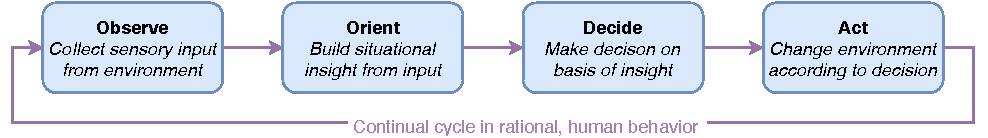
\includegraphics[width=\textwidth]{Figures/draw.io/underlying_concept_of_the_OODA_loop_by_Boyd}
    \decoRule
    \caption[Underlying Concept of the OODA Loop by Boyd]{Underlying Concept of the OODA Loop by Boyd.
    \textit{Source: figure 1 from \cite{Angerman2014} (edited), created with \href{https://www.draw.io/}{draw.io}}} 
    \label{fig:underlying_concept_of_the_OODA_loop_by_Boyd}
\end{figure}




%The functions of an autonomous UAV are:
%\begin{itemize}
%    \item "
%    \item Flight mission planning
%    \item Health condition monitoring
%    \item Fault detection, diagnosis, isolation and toleration
%    \item Missions and trajectories replanning which is according to insufficient battle information from sensors and data link
%    \item Autonomous take-off and landing
%    \item Flight attitude control, track following, payloads management and so on
%    \item Communication with ground station and other UAVs
%    \item The ability of dealing with unexpected situations
%    \item The ability of learning
%    \item "
%    \item application specific: surveillance, reconnaissance, remote sensing, target acquisition, border patrol, infrastructure monitoring, aerial imaging, industrial inspection, and emergency medical aid
%\end{itemize}
%


The hierarchical, autonomous control architecture for UAVs by Chen, Wang and Li \cite{Chen2009} (see figure \ref{fig:hierarchical_control_architecture_for_autonomous_UAV})
disaggregates the complex, autonomous control system of a generic UAV into three control levels (i.e., organization, coordination and execution level)
as well as a supervisor level for human intervention and an overlapping module for system monitoring.
By means of the IPDI (increasing precision with decreasing intelligence) concept, authority and tasks are distributed downwards.
In general, downstream from higher to lower levels, commands are distributed and system parameters are modified,
whereas command responses and preprocessed data are passed upstream from lower to higher level.
According to the outer/inner loop principle, higher control levels require longer intervals of planning and execution than lower control levels.

The most intelligent, least precise organization level implements artificially intelligent methods
that assess the situation and manage the mission, on the basis of the multi-sensor data from the coordination level,
and eventually, make decisions which are sent downstream to the coordination level.

The medium intelligent, medium precise coordination level runs conventional and artificially intelligent methods that, 
in accordance with the decisions from the organization level,
navigate and generate trajectories on the basis of multi-sensor data which is fusioned from preprocessed information sent by the execution level. 
Operational parameters are determined and, together with control and identification algorithms, are efficiently distributed to the subsystems of the execution level.

The least intelligent, most precise execution level directly interfaces with the sensors and actuators of the UAV. 
While receiving sensor data corresponding to the state of the UAV and the environment, 
this level runs conventional control algorithms (e.g., attitude, trajectory, velocity and propulsion control) with operational parameters as determined by the coordination level 
and sends low level control commands directly to the actuators of the UAV.
Moreover, this level runs identification algorithms that process the sensor data in order to determine parameters, to perform state estimation and to detect faults.
The gained information is sent upstream to the coordination level.

The supervisor level enables humans at the GCS to interact with the autonomous UAV.
However interaction is limited to the organization level, from where human commands are passed downstream.

The system monitoring module monitors the status and health information of all subsystems of the control system. 
In the occurrence of a fault, this module first, detects and localizes the fault
and second, modifies operational parameters in order to eliminate, reduce or tolerate the fault.
\begin{figure}
    \centering
    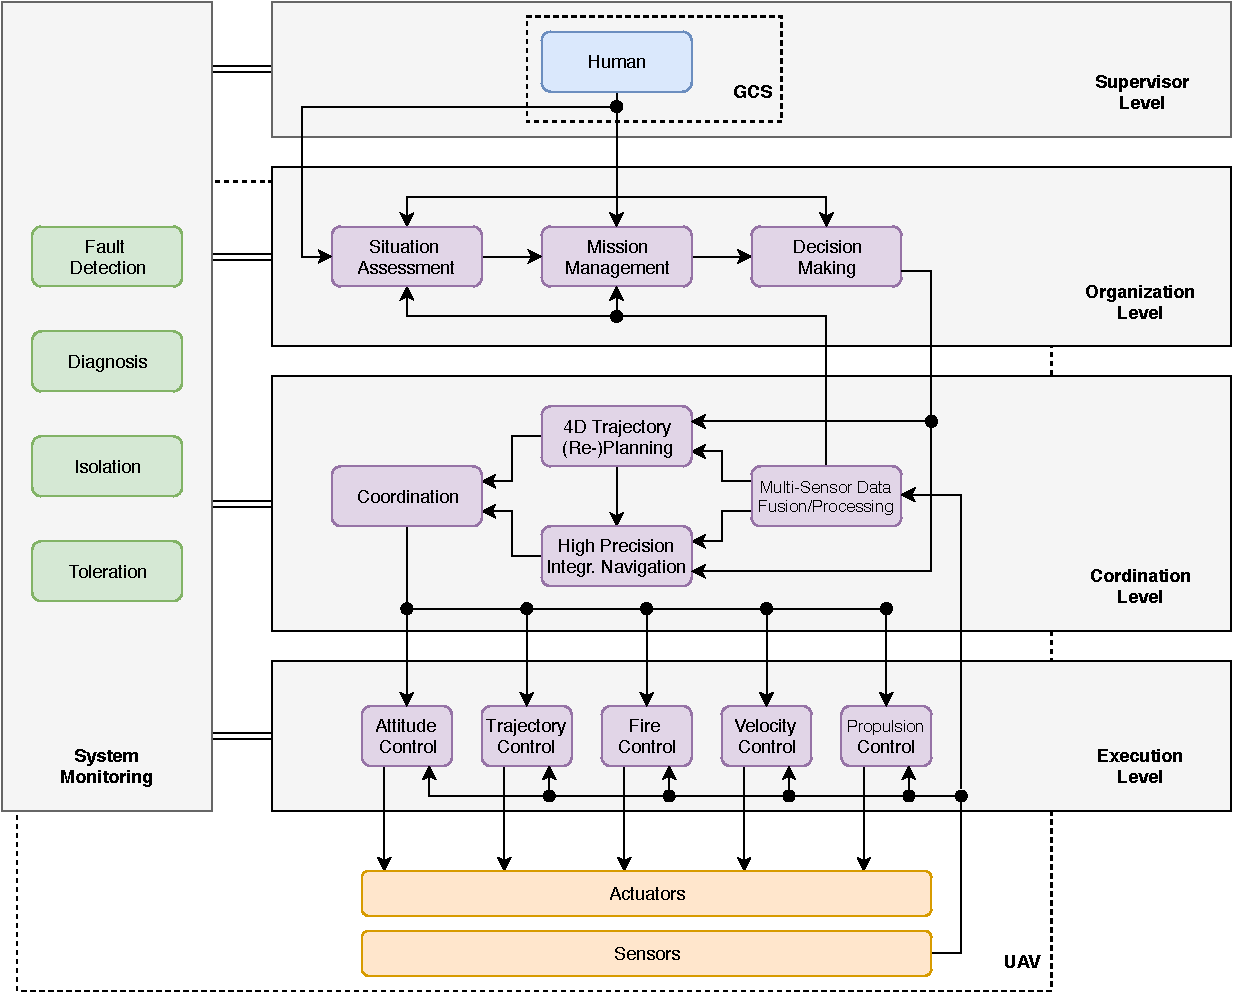
\includegraphics[width=\textwidth]{Figures/draw.io/hierarchical_control_architecture_for_autonomous_UAV}
    \decoRule
    \caption[Hierarchical Control Architecture of Autonomous Control for UAV by Chen, Wang and Li]{Hierarchical Control Architecture of Autonomous Control for UAV by Chen, Wang and Li \textit{Source: figure 2, 3 and 4 from \cite{Chen2009} (edited), created with \href{https://www.draw.io/}{draw.io}}}
    \label{fig:hierarchical_control_architecture_for_autonomous_UAV}
\end{figure}



%\paragraph{Navigation Control of MAVs}
%--------------------------------------------------------


%\cite{Chao2010} "Small  UAVs  normally  have  two  control  modes:  remote  control  (RC)  mode  and  autopilot  control  mode. 
% Remote  control  mode,  or  radio  control  mode,  requires  human pilots to control the UAV through radio signals, 
% while autopilot control mode can automatically keep the airplane at the desired state. 
% There are also mixed control modes  in  some  small  UAV  applications,  such  as  3400  Autopilot  from  UNAV  company. 
%  A  semi-autonomous  control  mode  is  provided  in  [8]  where  the  onboard  autopilot  controls  the  altitude  and  
%  the  human  operator  controls the flight path.
%" Although  RC  planes  can  be  applied  in  some  surveillance  situations, 
% the  full  concentration  of  an  experienced RC human operator is required all the time.
%  Therefore, autopilot systems are necessary to free human operators from tedious and repeatable jobs.
%   In addition, they  can  also  improve  the  navigation  accuracy  and  the  autonomy of UAVs.



%For the navigation of UAVs, there exist two general operation modes, i.e., the remote-controlled and the preprogrammed mode.
%The remote-controlled mode clearly linked to the concept of human operation,
%whereas the preprogrammed mode may range from automated to autonomous operation.
%
%The first two mentioned flight control modes are conventional, 
%whereas technologies related to the autonomous operation mode are rapidly evolving.
%
%In the \textbf{remote-controlled} operation mode, 
%a human pilot at the ground control station controls the flight of the UAV with a radio controller at all times.
%Thus, this operation mode requires an always reliable communication link between the ground control station and the UAV.
%Moreover, the maximum range of the communication link is a strict boundary for the flight range of the UAV and
%in certain environments (e.g., caves and mines) a reduced signal strength may make this operation mode completely infeasible. 
%This operation mode is mainly driven by the concept of human operation and exhibits related advantages and disadvantages.
%On the one hand, the awareness of the human pilot entails great flexibility with respect to situational changes and unexpected events.
%On the other hand, the limitations of human abilities also bound the flight performance of the UAV.
%A human has a limited reaction time which might be too long in an emergency case.
%Fatigue may appear during a long mission and shortens the flight endurance.
%Either a direct visual contact or a livestream from an onboard camera is required.
%Linear thinking prevents humans from applying complex mathematical optimization methods.
%Last but not least, human operation cause labor cost and relies on available, qualified workers.
%
%In the \textbf{preprogrammed} operation mode, an onboard computer controls the flight of the UAV
%according to a mission which has been uploaded to the onboard computer from the ground control station. 
%Refering to the concept of automation this operation mode benefits from the efficiency and accuracy provided by computation and complex, mathematical optimization.
%But it lacks of the comprehensive, situational awareness of a human.
%Thus, without human action preprogrammed UAVs cannot properly react to neither,
%significant changes of the overall situation that require mission updates, e.g., return to the ground control station if a storm come up,
%nor unexpected events within uncontrolled environments that occur during the preprogrammed mission, e.g., avoidance of a falling tree.
%Autonomy, as a combination of human reasoning and machine performance, is a major topic in current research on UAVs.
%Navigation of UAVs in the \textbf{autonomous} operation mode will overcome the above mentioned limitations inhered by both conventional operation modes.

%\textbf{Dynamics and Control}
%
%During flight, an UAV is an unstable system and requires continual control.
%Traditionally, this control is engineered on multiple control levels. \textbf{QUELLE} (except some end-to-end learning control methods).
%While on a lower control level, 
%an onboard autopilot is permanently maintaining attitude and altitude of the UAV in order to prevent collisions and keep up maneuverability,
%on a higher level, different actors can navigate the drone and perform maneuvers.
%Either a human pilot steers the UAV remotely from the GCS per radio transmitter (RC) 
%thereby, relying on direct visual contact to the vehicle  or on video stream from an onboard camera,
%or an onboard computer constantly executes algorithms to track trajectories thereby, relying on sensor data.
%While traditional navigation approaches, such as VIO or SLAM evaluate sensor data received from GPS, radio, inertial, SLAM, VIO to estimate the pose of the UAV,
%new approaches basing on camera or LIDAR data utilize perception concepts of machine learning.
%These computer tracked trajectories are either static, as part of a precomputed mission or adaptive to dynamic environments in sense of autonomous flight.
%
%However, even a remote-controlled UAV usually involves an autopilot 
%which supports the human pilot during flight by automatedly/autonomously performing tasks, e.g. maintaining pose.
%%and translation of higher order navigation tasks to individual lower level motor commands.





%\paragraph{Open questions}
%
%"It  is  shown  that  current  technologies  are  adequate  for  automated   UAV   
%that   operate   in   a   relatively   structured   environment.  
%For  UAV  in  a  rapidly  changing  uncertain  environment the present techniques are inadequate [2]." - \cite{Chen2009}
















































%\\\\\\\\\\\\\\\\\\\\\\\\\\\\\\\\\\\\\\\\
\section{Autonomous Navigation of MAVs}          \label{sec:autonomous_navigation_of_MAVs}
%////////////////////////////////////////

Autonomous navigation of MAVs is a current theme in recent research.
State-of-the-art methods are sophisticated, yet they fail in uncontrolled environments.
The current trend is to integrate deep learning into autonomous navigation methods
in order to give the MAVs perception and reasoning capacities.
Both abilities are fundamental for boosting the robustness of navigation methods 
which is necessary to cope with the uncertainty that occurs in uncontrolled environments.
MAVs fly at low attitudes in proximity to obstacles and other agents.
Moreover, they are restricted to lightweight sensors, computers and other devices
which strongly constrains applied navigation methods, that must realiably run in real time, in computational complexity.
Exspecially the sub-task of obstacle avoidance has remained highly challenging. \cite{Ross2013}

This section, first, examines the task of navigation in detail and identifies all sub-tasks.
Second, reliability and navigation qualities by which methods can be compared are discussed.
Third, the state of research on autonomous navigation for MAVs is reviewed.



%For humans, navigation through uncontrolled environments is part of everyday life, but for robots it has remained an unsolved task.
%
%
%Navigation is an essential task on every flight mission.
%It consists of three sub tasks that must be simultaneously performed by the MAV,
%i.e., to arrive at the target position (high level goal), 
%avoid obstacles and communicate with other agents in the environment. \cite{loquercio2018learning}
%
%
%
%
%According to Loquercio and Scaramuzza \cite{loquercio2018learning}
%the "safe and reliable navigation" of MAVs is a major unresolved obstacle for their application.

%--------------------------------
\subsection{Subdivision of Navigation}
%--------------------------------

\begin{figure}
  \centering
  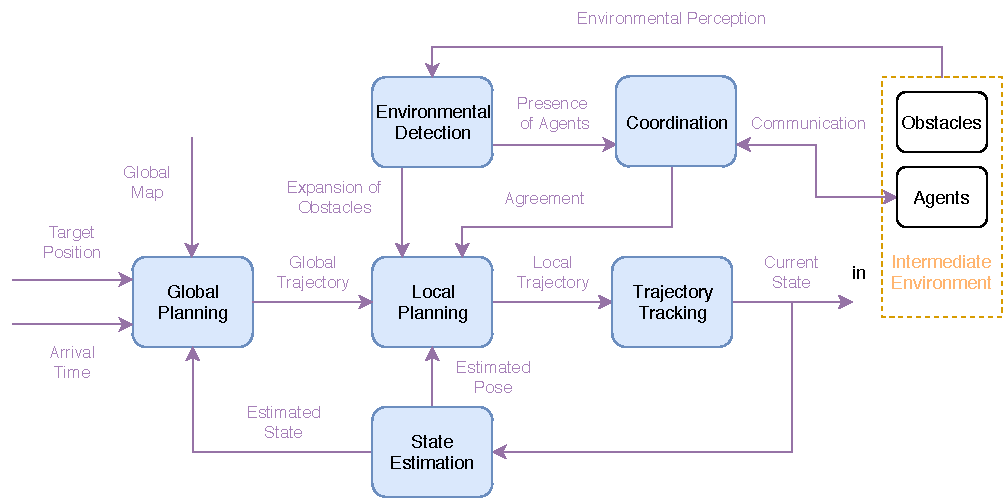
\includegraphics[width=\textwidth]{Figures/draw.io/sub-tasks_of_navigation}
  \decoRule
  \caption[The Sub-tasks of Navigation]{The Sub-tasks of Navigation. \textit{Source: own figure, created with \href{https://www.draw.io/}{draw.io}}}
  \label{fig:sub-tasks_of_navigation}
\end{figure}

The online dictionary Lexico.com \cite{Lexico.com-navigation} defines navigation as 
"the process or activity of accurately ascertaining one's position and planning and following a route".
The navigation task of a generic system may be devided into six continuos and simultaneous sub-tasks (see figure \ref{fig:sub-tasks_of_navigation}).
A sophisticated method for autonomous navigation should cover all of the sub-tasks.

The overriding goal of a navigation method is that the system to be navigated arrives at the target position at the desired time
as demanded by a higher-level unit (human operator or autonomous control structure).
Usually a map is used for this purpose.
First, the target position is identified in the coordinate frame of the map.
The current state (position, orientation and derivatives) of the system is estimated in the frame of the map.
A global trajectory in the frame of the map is generated 
that continuously connects the current state at the current time with the target position at the desired arrival time.
(Trajectories are 4D arrays consisting of consecutive 3D positions, each with a corresponding point in time and are
often calculated with optimization methods, for example, to minimize the distance travelled or the time required.)
Depending on the level of detail of the map, static obstacles may already be bypassed by the trajectory.
Based on the estimation of the current pose, 
the global trajectory in the coordinate frame of the map is converted to the local trajectory in the frame of the system.
The current, immediate environment is scanned to detect the expansion of obstacles 
and the presence of other agents in the frame of the system.
If necessary, communication with other agents is established to coordinate further motion.
In case of conflicts, the local trajectory is adjusted to avoid the obstacles or to follow the agreement with the other agents
but to still follow the rough course of the global trajectory.
Finally the collision-free trajectory is tracked by accordingly move the system.

All the above actions are performed more or less simultaneously and constantly.
At all time the current state of the system is estimated. 
If at any time this estimation essentially differs from the global trajectory or changes occur in the map, 
the global trajectory may be re-planned.
Since the system is continuously changing its state, the global trajectory is constantly converted to the local trajectory in the frame of the system.
The system must perceive the environment and may adjust the local trajectory at all times 
in order to be able to cope with unpredictable, dynamically moving obstacles and agents.
Simultaneously, the system must continuously follow the trajectory.

Considering the complexity, it is admirable how humans can accomplish the navigation task without much effort.
The street scenes of their residential areas may be the map stored in their mind.
They may estimate their current state based on their vision of the immediate environment
and transfer the global trajectory to the frame of their own body.
While continuously walking along the local trajectory,
at ease, they properly react to red traffic light, puddles, other pedestrians, etc.
From experience, they may choose alternative routes accordingly to the current situation and
know how to adjust their walking speed to arrive at the desired time.







%------------------------------------------------------
\subsection{Reliability and Qualities}
%------------------------------------------------------

Lazzaroni, Cristaldi, Peretto, Rinaldi and Catelani \cite{Lazzaroni2011}
define reliability of a system as the "probability [...] of performing its required function 
in the established time interval, under established conditions".
In the context of autonomous navigation of MAVs,
the required function is to safely fly to the target position.
Thereby, the time interval is established by the desired arrival time.
Depending on the intended application, the time interval may be short requiring the MAV to navigate at high speeds.
For this, not only the flight control system of the MAV but also the navigation method must be highly agile.
The conditions are determined by the intended application environment through which to be navigated and the design of the MAV.
Depending on the application environment, the navigation method must integrate certain sub-functions to ensure safety.
The design of the MAV constrains the capacities of electric and computation power available for the navigation method.

This subsection discusses the impact of functional scope, efficiency and agility
of autonomous navigation methods for MAVs on their reliability, 
i.e., the probability that the navigation method performs 
the required function (safely navigate to the target position in time)
in a certain environment, with certain ressources, in a certain application.
Functional scope, efficiency and agility can be considered as qualities
which are applicable in the development of autonomous navigation methods for MAVs and the comparison of their performance.


\paragraph{Functional scope}
%----------------------
The application environment poses which sub-functions of navigation (see figure \ref{fig:sub-tasks_of_navigation}) 
are required to be integrated into the navigation method.
In controlled and undisturbed environments, such as the airspace of rural areas,
navigation methods may be considered reliable without the ability to perceive and reason the immediate environment
since the environment is highly predictable.
In contrast, uncontrolled environments which may be unstructured and dynamically variable and 
in which multiple agents may simultaneously act, exhibit substantial uncertainty.
An example is the traffic environment in urban areas, in which a large number of different road users participating. 
Those uncontrolled environments demand the robust performance of all sub-tasks of navigation.
The lack of structure, dynamic changes and multiple simultaneously acting agents
may be too complex to be fully captured on global maps.
For example, maps may show the position of a tree or an other agent but not the tree's branches or the agent's next movement.
Thus, the MAV must be able to detect the expansion of the tree and the presence of the agent,
in order to locally re-plan or coordinate a collision-free trajectory.
Environments with highly dynamical obstacles may require a high agility for
the navigation method for fast reactions.


\paragraph{Efficiency}
%-----------------------------------
In the design of MAVs, hardware components are severely limited in size and weight
which in turn strongly constrains power capacities and computational power.
Bigger batteries and processors would sensitively affect the size and weight of the MAV 
and thus, may decrease the maneuverability and agility of the MAV. \cite{Verbeke2017}
Therefore, navigation methods are required to be energetic and computational efficient.
Methods are only reliable, if they are processable in real time by the constrained hardware.
The navigation system may be a significant electricity consumer of the MAV.
The less energy the navigation system requires, the more energy is available for longer flights and payload.
Autonomous navigation methods may essential differ in energy consumption by the type and number of sensors they are based on
as well as their computational complexity which determines the processor performance required to run them in real time. \cite{Chao2010}


\paragraph{Agility}
%--------------------------------------
The online dictionary Lexico.com \cite{Lexico.com-agility} defines agility as the capability,
first, "to move quickly and easily" and, second, "to think and understand quickly".
In the context of aviation, agility is closely linked to maneuverability. 
Both are "flight qualities" \cite{Whalley1991} that find application in aircraft design.
Lawrence, Corning and Wharburton \cite{Lawrence1991} define
maneuverability as the "ability to change the aircraft flight path by application of forces from the main rotor, 
tall rotor or other control devices"
and agility as "how quickly the aircraft flight path can be changed".
Whalley \cite{Whalley1991} measures maneuverability/agility of an aircraft by
"the maximum achievable time-rate-of-change of the velocity[/acceleration] vector".
Accordingly, maneuverability and agility encompass the execution control and dynamics of an aircraft
and reflect the first part of the definition of Lexico.com.

MAVs are generally very agile due to their small size.
However, their agility is very sensitive to their weight and is therefore in a strong conflict with higher endurance and payloads. \cite{Verbeke2017}
Agility often suffers in favor of safety which is the top priority of autonomous navigation.
In contrast to professional human pilots,
autonomous navigation control methods have not yet been able to push the dynamics of MAVs safely to the limit. \cite{Kaufmann2018}
Exspecially with navigation methods based on global state estimation, high speeds easily leads to failure. \cite{loquercio2018learning}
For a better comparability of autonomous navigation methods, it may be advisable to extend the above definitions of maneuverability and agility 
to the second part of the definition of Lexico.com.
Agility in the context of autonomous navigating MAVs should not only include the execution control level (see figure \ref{fig:hierarchical_control_architecture_for_autonomous_UAV})
and the dynamics of the airframe but also the autonomous navigation control.
In this case, all steps of the OODA loop (see figure \ref{fig:underlying_concept_of_the_OODA_loop_by_Boyd}), 
i.e., to observe, orient, decide and act, would be covered by the extended concept of agility.








%------------------------------
\subsection{State of Research}
%------------------------------

The development of comprehensive, autonomous navigation methods for MAVs is complex 
because the method must integrate several functions that perform simultaneously running sub-tasks (see figure \ref{fig:sub-tasks_of_navigation}).
Loquercio and Scaramuzza \cite{loquercio2018learning} categorize the numerous existing autonomous navigation methods for MAVs
into classical methods that follow the scheme of mapping-localization-planning-tracking,
and modern methods which, with the use deep learning, train the MAV to learn end-to-end navigation policies.
In turn, they subdivide deep learning methods into methods based on imitation learning and reinforcement learning.
%% FERTIG
%They point out that classical methods for autonomous navigation of robots are not robust enough for safe use in uncontrolled environments
%since they are based on global state estimates that cannot respond adequately to dynamics and unpredictability (see ???).
%Recent research integrates deep learning to enable perception and awareness. 
%Methods here are not mature yet but have the long-term potential to solve uncontrolled environments for autonomous navigation (see ??).
Following the classification of Loquercio and Scaramuzza, 
this section presents the state of research on autonomous navigation methods of MAVs and discusses advantages and disadvantages.


%SLAM
%visual aliasing
%dynamicscenes,  and  strong  appearance  changes
%
%end-to-end: "bond perception and control.[6][7], [8], [9]" \cite{loquercio2018learning}
%
%policy: "
%A policy is a state-action mapping. 
%A 'state' is a formalism used in AI that represents the state of the world, i.e. what the agent's idea of the world is. 
%The action is, naturally, what action it should take in that state. A policy just maps states to actions.
%"
%%https://datascience.stackexchange.com/questions/27016/what-is-a-policy-in-machine-learning
%
%imitation 
%
%reinforcement


\paragraph{Classical methods}
%----------------------------

Traditionally, navigation methods follow the the scheme of intermeshed steps, i.e., mapping-localization-planning-tracking.

A common and simple type of system architecture for the navigation of MAVs through undisturbed outdoor environments
estimates the state of the MAV based on data from an onboard GNSS sensor and localizes the MAV in a given map.
Based on the current position of the MAV, the target position and the information of the map, a trajectory is generated and tracked.
This type has two main disadvantages.
First, in environments where the GNSS signal may be weak, as for example in urban areas, GNSS based navigation methods are not reliable.
Second, functions to cope with obstacles and other agents in the immediate environment are absent.

More sophisticated system architectures integrate simultaneously localize and mapping (SLAM) algorithms, 
which do not require GNSS signals but visual or range sensors.
SLAM algorithms generate and update a map of an unknown environment which captures present obstacles and 
simultaneously localize the system in the map. \cite{Mur-Artal2015}
Path planning algorithms (e.g., \cite{Bircher2016}, \cite{Cieslewski2017}) 
identify collision-free trajectories in 3D depth maps build by the SLAM algorithm.
Sophisticated navigation methods for MAVs exist that estimate the MAV state based on data from an inertial measurement unit (IMU)
together with the output of vision-based SLAM algorithms (e.g., \cite{Lin2017}, \cite{Scaramuzza2014}, \cite{Sa2018}, \cite{Loianno2017}).


The main disadvantage of SLAM methods is that generating the map of the environment coerces global consistency.
This increases computational complexity and causes extreme effort to capture the dynamics of environments.
Thus, classical methods reach their limits in environments which are not pre-dominantly static, i.e., fast changes may occur.
Moreover, they are prone to fail at high speeds due to visual aliasing.
In contrast to end-to-end policies, classical methods are a compound of clearly separated sub-systems.
As a result, possible positive feedback effects between perception, reasoning and control 
are prevented in the first place and one-way, complex algorithms must be deployed to
connect the sub-systems by generating control commands based on 3D maps.








\paragraph{Methods based on deep reinforcement learning}
%--------------------------------------------------

%"robot experience" ?? experience = learning?

Recent Research has publicated various navigation methods involving deep reinforcement learning (RL) algorithms.
Automatically generated control policies input raw sensor data and output complex flight control commands.
%[9],  [25],  [26].
RL Navigation methods are vision- or range-based, 
i.e., they input images of a video camera or depth maps (at each pixel the distance to an object) of a LiDAR.
The foremost benefit of deep RL methods is that policies are not affected by the control shift problem that occurs with IL methods,
because the policies are learned with "trial-and-error" \cite{Sadeghi2016} from direct environmental interaction without the need for expert intervention.

However, this way of learning requires an enormously high degree of sample complexity to achieve generalizing policies. \cite{Zhu2017}
For MAVs, limited flight endurance makes the learning process inefficient. \cite{Sadeghi2016}
Moreover, any collision is highly uncontrolled and thus very likely critical for the health of the system and the safety of the environment. \cite{Sadeghi2016}
Thus, to acquire the required sample complexity is extremely costly and dangerous. 
Researchers tried to circumvent this by transferring part or all of the learning process to simulation 
while still testing the learned policies in the real world. 

Sadeghi and Levine \cite{Sadeghi2016} propose a vision-based policy for collision avoidance in real world indoor flight 
which is exclusively trained with simulated training data.
From raw monocular RGB images, a deep convolutional neural network directly outputs velocity motor commands.
A variety of higly randomized environments, textures and lighting, produces control policies that generalize to the real world.
In real world test flights, they prove collision-free navigation through indoor environments. 
But the MAV flies with extremly low agility.

State-of-the-art simulation environments are capable of comprehensively modelling the dynamics of a quadcopter MAV. \cite{Meyer2012}
Nevertheless, open problems have not been solved yet.
First, complex aerodynamic effects such as rotor drag, which become important with the flight close to structures, is not yet be modelled. \cite{Faessler2018}
Second, learned policies are affected by a domain shift between simulation environments and the real world.
Even in the presence of photorealistic simulators (e.g., AirSim \cite{Shah2017}, CARLA \cite{Dosovitskiy2017}),
the quality of rendered images is not yet sufficient.
Zhu, Mottaghi, Kolve, Lim, Gupta, Fei-Fei and Farhadi \cite{Zhu2017} address the domain shift by fine-tuning 
their vision-based deep RL policy learned in simulation with training data from the real world.












\paragraph{Methods based on deep imitation learning}
%---------------------------------------------------


%end-to-end policies may closely link perception, reasoning and control.

%Recently, new approaches based on  deep  learning  have  offered  a  way  to  learn  end-to-end flying  policies,  
%tightly  coupling  perception  and  control  [6],
%"Exspecially, methods based on supervised learning are promising 
%"since  they  offer  an  effective  and sample efficient way to learn flying policies".
%Nevertheless, the domain shift between teacher and learner is challenging." \cite{loquercio2018learning}


Over the last years, more and more research has been done on methods of autonomous navigation
that involve deep imitation learning in order to learn control policies from raw sensor data, usually camera images or depth maps.  %[6], [7], [19], [8],[20], [21]. 
Compared to reinforcement learning, imitation learning is easier to implement and characterized by a low sample complexity. 
This means that smaller amounts of training data are necessary to generalize learned control policies to test scenarios.
However, the collection of training data as well as the evaluation of learned control policies
may be inefficient and dangerous, exspecially in uncontrolled environments.
Therefore, some researchers have chosen alternative ways to collect training data.
Loquercio, Maqueda, del-Blanco and Scaramuzza \cite{Loquercio2018} trained a deep neural network 
with real world data that has been safely gathered by cars and bicycles driving through urban areas.
They achieved a generalized control policy 
that also could safely navigate the MAV at high altitude in urban areas and also through indoor environments.
Similarly, Giusti, Guzzi, Cirsan, He, Rodríguez, Fontana, Faessler, Forster, Schmidhuber, Di Caro, Scaramuzza and Gambardella \cite{Giusti2016}
as well as Smolyanskiy, Kamenev, Smith and Birchfield \cite{Smolyanskiy2017} used image data collected by human hikers.
The derived control policies could safely navigate MAVs through forest trails.
Alternatively, the learning process can be shifted to simulation, i.e., train the network on simulated data (see next paragraph).

Many navigation methods are restricted to planar motion not exploiting the agile dynamics of MAVs.
Ross, Melik-Barkhudarov, Shankar, Wendel, Dey, Bagnell and Hebert \cite{Ross2013}
developed a navigation system that inputs images from a monocular camera and
reactively controls the MAV in planar motion in order to avoid trees.
The policy, in the form of visual feature extraction plus a neural network is trained to mimic yaw control of human pilot experts.
They could demonstrate collision-free flight with velocities up to 1.5 $\frac{\text m}{\text s}$
in a controlled indoor environment as well as in outdoor forest environments.
Giusti et al. \cite{Giusti2016}  used a deep convolutional neural network to map images
to the direction of forest trails relative to the MAV.
They could achieve a classification accuracy that is comparable to human decision.
However, the flight control of the MAV was restricted to planar motion (i.e., yaw and speed control)
The convolutional neural network of Loquercio et al. \cite{Loquercio2018}
outputs a steering angle and a collison probability.
The policy can follow roadways and simultaneously avoid obstacles
but is also limited to planar control, i.e., forward velocity and yaw control.




%Loquercio and Scaramuzza \cite{loquercio2018learning} name the main disadvantage of 
%neural network policies to be the "lack planning to reach high-level goals"
%and the "control-shift  between  the expert providing supervision and the learning agent" 
%Thus, state-of-the-art deep IL methods are often limited in their maneuverability
%(e.g., they only control planar motion) as well as in their agility, i.e., 
%the UAVs move timidly and jerkily so that they do not make use of their possible flight dynamics.
%
%... propose a hybrid method that combines IL with conventional model-based control algorithms.
%The vision-based policy is able to navigate the UAV with high agility.
%In addition, generalization is achieved with a relatively low sample complexity.


%\cite{Ross2013}
%input: monocular RGB images from onboard forward facing camera.
%processing: vector of visual featuresxfromthe current image, 
%  neural network with ridge regression, imitation learning, smallset of human pilot demonstrations, 
%  ontroller that canavoid trees by adapting the MAVs heading
%output:  left-right velocity control commands,  fixed  forward velocityand altitude
%success: navigates a small quadrotor helicopter autonomously at low altitude through natural forest environments
%  maintain a constant velocity of up to 1.5m/s
%  demonstrate theperformance of our system in a more controlled environmentindoors, and in real natural forest environments outdoors.
%mentionable: planar motion
%  -:


%\cite{Giusti2016} 
%input: monocular RGB  images from onboard forward facing camera
%processing: deep neural network as supervised image classifier
%output: heading of the forest/mountain trail with respect to the viewing direction.
%success: classification accuracy comparable with humans, outperforming of then state-of-the-art methods
%mentionable: planar motion, quadcopter MAV with implemented system (Yaw and speed control) can navigate unseen forest trail
%-: agile dynamics of drones is not fully exploited
%  not directly possibleto explicitly give the robot a goal to be reached, as it iscommon in other CNN-based controllers


%\cite{Loquercio2018}
%input: monocular RGB  images from onboard forward facing camera
%processing: DroNet, convolutional neural network, 8-layers residual network
%output: steering angle to keep the drone navigating while avoiding obstacles-ollow the roadway; 
%  collision probability to let the MAV recognize dangerous situations and promptly react to them- react to dangerous situations exactly as any other groundvehicle would do
%success: generalize policy, MAV at relatively high attitude, indoor environments (parking lots, corridors);
%  safe flight of a quadrotor in urbanenvironments, new application spaces without anyinitial knowledge,
%   scenarios completely unseenat training time including indoor corridors, parking lots,and high altitudes.
%   ater converted into control flying commands
%mentionable: train a MAV from data collected bycars and bicycles, planar motion with forward velocity (2nd output) and yaw (steering angle)
%-: agile dynamics of dronesis not fully exploited
%  not directly possibleto explicitly give the robot a goal to be reached, as it iscommon in other CNN-based controllers



%\cite{Smolyanskiy2017}
%
%input: monocular image
%processing: deep neural network
%output: view  orientation  and  lateral offset  of  the  MAV  with  respect  to  the  trail  center
%success: autonomously following trails in unstructured, outdoor environments such asforests
%  DNN-based  controller  achieves  stable  flight  without  oscillations,  smoother 
%  autonomous  flights  of  1  km
%-: agile dynamics of dronesis not fully exploited???
%not directly possibleto explicitly give the robot a goal to be reached, as it iscommon in other CNN-based controllers
%mentionable: increase robustness with 2 additional vision systems: DNN  for  objectdetection and 
%  visual  odometry  component  for  estimatingdepth for the purpose of low-level obstacle detection
%
%
%
%Smolyanskiy et al. \cite{Smolyanskiy2017}





%[20] "The supervisory signal comes from hard-coded trajectories"  
%
%
%How do you learn to navigate an Unmanned AerialVehicle  (UAV)  and  avoid  obstacles? 
%One  approach  is  to  usea  small  dataset  collected  by  human  experts: 
% however,  highcapacity learning algorithms tend to overfit when trained withlittle  data.  
% An  alternative  is  to  use  simulation.  
% But  the  gapbetween simulation and real world remains large especially forperception  problems.  
% The  reason  most  research  avoids  usinglarge-scale  real  data  is  the  fear  of  crashes!  
% In  this  paper,  wepropose to bite the bullet and collect a dataset of crashes itself!
% We build a drone whose sole purpose is to crash into objects: 
% itsamples naive trajectories and crashes into random objects.
%  Wecrash our drone 11,500 times to create one of the biggest UAVcrash dataset. 
%  This dataset captures the different ways in whicha  UAV  can  crash.  
%  We  use  all  this  negative  flying  data  in  con-junction 
%  with positive data sampled from the same trajectoriesto  learn  a 
%   simple  yet  powerful  policy  for  UAV  navigation.  
%   Weshow that this simple self-supervised model is quite effective innavigating  
%   the  UAV  even  in  extremely  cluttered  environmentswith  dynamic  obstacles  including  humans.
%
%
%
%[21] The supervisory signal comes from model predictive control
%
%neural network architectures  [8], [23], [24]























%\paragraph{Unsolved Issues}
%%--------------------------
%
%<
%There  has  been  many  significant  research  in  making  UAV  fly  autonomously,  
%but  obstacle  avoidance  is  still  a  crucial   hurdle.   
%For   small   quadrotor   UAV,   due   to   the   limitation  of  payloads 
% it  is  infeasible  to  carry  sophisticated  radar  sensors.  Though  many  advanced  research  
% has  used  light  detection  and  ranging(LiDAR)  [1]  or  the  cameras  of  Microsoft Kinect [2], both sensors are heavy, 
% which will lead to  increase  the  power  consumption  and  drastically  decrease  the flight time.
%>
%\cite{Ross2013}
%
%<
%"Even though systems based on deep learning achieve remarkable  results,  
%we  believe  that  those  systems  are  still not  ready  to  completely  replace  traditional
%  “map-localize-plan” approaches for drone navigation. 
%Indeed, we speculate that  learning-based  and  traditional  approaches  are  going  to
%  complement each other and enable drones to accomplish the most challenging tasks."
%>
%\cite{loquercio2018learning}
%
%
%High Level Goal formulation






























%\subsection{+Autonomous Navigation Systems for Small Quadcopters}
%Flight Control Pipeline
%
%
%\paragraph{Classical System Architecture}
%Env - Sensor - State (Velocity) Estimation                              - Velocity Controller - Flight Controller - Motors
%             - obstacle detection - local planner - position controller -














 
% Chapter Template

\chapter{The Research Project} \label{cha:research_project} % Change X to a consecutive number; for referencing this chapter elsewhere, use \ref{ChapterX}

For my master thesis within the  
"Double/Joint Degree Master Program in Mechanical Engineering/Physikalische Ingenieurwissenschaft 
of Tsinghua University and the Technical University of Berlin",
I decided to research on the topic "\ttitle".
This chapter, first, clarifies the objective of the research of this master thesis and
discusses the potential contribution to the field of autonomous navigation of UAVs.
Secondly, the intended methodology and elaboration of
the general design of the unmanned aerial system, the navigation system and the test scenario, is presented.
Thirdly, the scope of this master thesis is reflected in a schedule of research and thesis writing.






%While the methods can successfully avoid obstacles,
%they lack of a high-level goal formulation and lose orientation if there is nothing to react to.
%High-level formulation is an inherent problem for deep learning.
%Within my research, I aim to develop an autonomous navigation method for MAVs that can bridge phases without orientation
%by empowering the MAV with power of recall.
%Trained with imitation learning, the policy should map not only the current image 
%from a forward facing camera but also selectively remembered, elapsed images to current actions.
%Then, the MAV could not only perceive in the spatial but also in the temporal dimension, i.e., remember,
%which in turn would make the navigation method robust against phases without orientation.





%-----------------------------
\section{Research Objective and Anticipated Contribution}
%-----------------------------

Although many sophisticated methods for the autonomous navigation of MAVs already exist,
open-world environments of high uncertainty have not yet been conquered by autonomous MAVs (see section \ref{sec:autonomous_navigation_of_MAVs}).
Current research is making effort to face the uncertainty of these environments by using deep learning techniques 
that empower MAVs with necessary perception and reasoning abilities.
State-of-the-art, vision-based navigation methods integrate policies in the form of feedforward, deep convolutional neural networks
that map the current state in form of the current picture to action.
Convolutional neural networks already achieve a high, spatial perception and reasoning of the immediate environment, however, 
this alone may not be enough for the long-term objective to robustly apply autonomous MAVs in open-world environments.

Kaufmann, Loquercio, Ranftl, Dosovitskiy, Koltun and Scaramuzza\cite{Kaufmann2018}
developed a vision-based method that navigates a MAV through a drone racing track with possibly dynamically moving race gates.
Thereby, they achieved a high reliability and agility at high speeds.
But the method, exemplarily of other methods, has a decisive deficiency that stands out 
due the inherent problem of high-level goal formulation in deep learning.
At any time, the next gate must be in the frame of view (FOV) of the onboard camera. 
If not, the navigation method has no target position.
This is also the case, even if the MAV has seen the next gate in the past.
For example, a section of the racetrack that consist of two successive gates, in between a steep curve
could not successfully be navigated through by the method, even if both gates have already appeared on images.
Before the MAV navigate through the first gate, both gates are in the FOV of the camera.
After it has flown through the first gate, because the curve is too steep, the second gate is out the FOV 
and the navigation method has no goal to be achieved.

The lack of high-level goal planning is an inherent problem of deep learning policies.
In the navigation method of this research, I want to meet the lack of high-level goal planning 
by introducing powers of recall to navigation.
To my knowledge, Kelchtermans and Tuytelaars \cite{Kelchtermans2017}
are the only ones who used a recurrent neural network for memory abilities in autonomous, vision-based UAV navigation. \cite{Shakeri2019}
However, they only tested their method in simulation and did not comprehensively evaluate their results.
If the method, after passing the first gate, could remember that it has seen the second gate before,
the method could plan to navigate through the second gate based on elapsed images.
% HUMAN IN THE DRONE RACETRACK EXAMPLE
%To solve this problem I consider what a human would do in this scenario.
%From a position before entering the gate 1, a human can see gate 1 and 2.
%After he flew through gate 1, he has no visual contact to both gates anymore.
%Yet, he can manage to navigate through gate 2 because he has the ability 
%to remember the position of gate 2 in his body frame. 

Deep learning enables machines to learn human-like abilities of perception and reasoning.
Thus, it seems promising to orient methods also on human behavior.
Powers of recall in human navigation has an important function.
For example, after entering a room, humans can still locate themselves relatively to the door which is not in their FOV anymore.
In addition, humans cannot estimate the velocity and direction of motion of themselves, obstacles or other agents
based on a short blink with their eyes but they need to observe over at least a short period of time.
Not only localization but also situational reasoning is strengthened by memory,
e.g., a car driver observes a child that runs from the sidewalk through the parking cars onto the road
and has enough reaction time or even anticipation to brake.
Without any power of recall, the driver may start braking in anticipation
when the child is still on the sidewalk, but may stop braking after the child disappears behind a parking car.

In my method, I plan to use deep convolutional neural networks serially connected to a long-short-term-memory (LSTM) neural network.
While the CNN has the ability to perceive and reason spatial structures of the environment,
the LSTM is able to establish connections through time. 
In other words, the CNN is responsible to predict waypoints or generate trajectories based on single images,
whereas the LSTM empower the method to recall and remember by evaluating the temporal structure between the predictions of the CNN.
Besides the above steep curve scenario, this memory would show great benefit in situations
when the quadcopter lost track of the goals and he can recall elapsed images.
In case of the application in urban areas, for example, 
quadcopters could remember obstacles that were visible but have become occluded and thus, could better anticipate. 
Or after an evasive maneuver, the quadcopter could return to the actual path much faster because he memorizes its maneuver.
In that sense, the memory of the quadcopter is another form of localization in the environment, which is not global but namely local.
In addition, memory could enable better optimization, e.g., the imitation learning of optimal trajectories which
are not only spatial but also temporal objects.
However, this research, in a simplified scenario, should only prove if powers of recall are applicable and generally useful 
for the autonomous navigation of MAVs.









%LSTM - MEMORY PAPER%https://arxiv.org/pdf/1702.07600.pdf
%OVERVIEW PAPER %https://arxiv.org/pdf/1810.09729.pdf


%occlusion, small field of view effects, Figure 7: \cite{Ross2013}
%
%
%
%They also use PX4.%https://arxiv.org/pdf/1705.02550.pdf




















%\\\\\\\\\\\\\\\\\\\\\\\\\\\\\\\\\\\\\\
\section{Methodology and Elaboration}
%//////////////////////////////////////


%----------------------------
\subsection{Setup of the UAS}
%----------------------------

The GCS is represented by a laptop, a wireless LAN router as ground data terminal and an RC controller for emergency cases.
At the GCS, the human operator switches on/off and arms the MAV as well as sets the flight control mode to preprogrammed (normal operation)
or to remote-controlled (emergency case).
In the preprogrammed mode, the human operator only supervises the autonomously navigating MAV and
the navigation control system autonomously controls the MAV as described in the next subsection.
In the remote-controlled mode, 
the human operator manually sends navigation commands (e.g., turn left, assume the pose) via the RC controller
to the RC receiver of the air data terminal onboard the MAV.
The flight controller tracks those navigation commands while also stabilizing the MAV
by sending out corresponding low-level control commands  to the individual actuators of the flight control system of the MAV.





%---------------------------------------------------
\subsection{Design of the Navigation Control System}
%---------------------------------------------------

The navigation control system of this thesis builds on the navigation methods of Kaufmann et al. \cite{Kaufmann2018}.
Similarly, the system is subdivided into the perception/reasoning, the path-planning and the low-level control system.
While the path-planning and the low-level control system remain broadly the same,
the perception/reasoning system is structurally oriented towards the design of Kelchtermans and Tuytelaars \cite{Kelchtermans2017},
i.e., the serial connection of a CNN and a LSTM network that can perceive and reason in both the spatial and temporal dimension.
However, instead of using the CNN to extract generic features from images like Kelchtermans and Tuytelaars,
the CNN maps images to a higher level representation in the form of waypoints and desired velociy 
similarly to original approach by Kaufmann et al. \cite{Kaufmann2018}.
With this, I aim to significantly reduce computational costs in comparison to Kelchtermans and Tuytelaars
while remaining the agility qualities of the method of Kaufmann et al. \cite{Kaufmann2018}.


The perception/reasoning system is a serial connection of a deep convolutional neural network and a LSTM network.
The CNN policy inputs the current image from the forward-facing onboard camera of the MAV
and outputs for each of the next two gates a waypoint in the images coordinates as well as a corresponding normalized speed.
\begin{align}
    \left\{ \vec x_i \in [ -1,1 ]^2 \in \mathbb{R}^2 ,\ v_i \in [0,1] \in \mathbb{R} \right\} ,\ i=1,2
\end{align}
If the image does not depict gate $i$, the corresponding normalized speed is zero, i.e.,
if there is no gate, both velocities are zero;
if there is one gate, the first velocity is a non-zero value and the second velocity is zero;
if there are two gates, both velocities are non-zero values.
\begin{align}
    v_i \in
    \begin{cases}
        \{0\},\ &\text{if picture does not depict gate }i \\
        ]0,1],\ &\text{else} 
    \end{cases}
    \quad,\ i=1,2
\end{align}
Indices $i=1/2$ refer to the closer/farther one of two closest gate, 
which is detected by the expansion (e.g., area or diameter) of the gates on the image.
In case there are more than two gates in the picture, the gates besides the closest two are neglected.
Assuming that in a common racetrack the next gate is also the closest gate,
indices $i=1/2$ correctly reflect the sequence of the race gates in the racetrack.


The LSTM policy inputs the output of the CNN network as well as acceleration data from onboard sensors.
In case that the current image depicts one or two race gates (i.e., $v_1 \in ]0,1]$),
the LSTM directly outputs $\vec x = \vec x_1,\ v= v_1$ to the path-planning system.
In case that the current image depicts no race gate (i.e., $v_1 = 0$),
the LSTM outputs a bridging waypoint $\vec x = \vec x_b$ with a corresponding bridging velocity $v=v_b$.
\begin{align}
    \left\{
    \vec x = 
    \begin{cases}
        \vec x_1\ & \text{if }v_1 \in ]0,1] \\
        \vec x_b\ & \text{else}
    \end{cases},\ 
    v =
    \begin{cases}
        v_1\ & \text{if }v_1 \in ]0,1] \\
        v_b\ & \text{else}
    \end{cases}
    \right\}
\end{align}
Assuming the next gate had been depicted before the MAV has navigated through the last race gate,
the relative position of the next gate to the unaccelerated MAV can be estimated by the course of
the elapsed waypoints of the farther gate (i.e., $\vec x_2$) before the gate had left the FOV (i.e., before $v_2 = 0$).
However, the MAV has been accelerated in the meantime.
Therefore, the LSTM also inputs the acceleration data in order to estimate
the additional, relative displacement of the race gate due to acceleration of the MAV since the gate has left the FOV.
This bridging navigation is required to be too accurate because the goal is that the race gate, 
that has disappeared in the meantime, re-appears in the FOV of the camera.
Then again, the LSTM only passes the predictions from the CNN as described.

The path-planning system inputs the waypoint $\vec x$ in image coordinates and the normalized velocity $v$.
First, the actual speed is computed with the maximum velocity $v_{\text{max}}$ which is set by the human operator 
to determine the maximum and therewith also average speed of the MAV.
\begin{align}
    v_{\text{out}} = v_{\text{max}} \cdot v
\end{align}
Secondly, the prediction horizon is determined proportionally to the velocity $v_{\text{out}}$,
however, in the range $[d_\text{min}, d_\text{max}]$.
The proportionality factor $m_d$ as well as the range parameters $d_\text{min}$ and $d_\text{max}$
are set by the human operator to influence the aggressiveness of the flight of the MAV.
A smaller prediction horizon at lower speed allows agile flight required in sharp curves,
whereas a bigger prediction horizon at higher speed smoothens the flight which is beneficial on straight racetrack sections.
\begin{align}
    d = \text{min} \{\text{max}\{d_\text{min}, m_d \cdot v_{\text{out}}\}, d_\text{max}\} 
\end{align}
Thirdly, the waypoint $\vec x$ in image coordinates 
is transformed to the waypoint $\vec p = (p_1, p_2, p_3)^T \in \mathbb{R}^3$ in the coordinate frame of the MAV.
The x-component is set equal to the prediction horizon (i.e., $p_1 = d$).
With a back-projecting transformation $T$ of a library (e.g., OpenCV \cite{OpenCV}) the y- and z-components are computed.
\begin{align}
    \vec p &= (p_1, p_2, p_3)^T \in \mathbb{R}^3 \text{ with } & p_1 &= d \nonumber \\
    && (p_2,  p_3)  & = T\left\{ \vec x\right\}
\end{align}
Fourthly, a computationally efficient, minimum-jerk trajectory segment $t_s$, 
as proposed by Mueller, Hehn D'Andrea \cite{Mueller2013}, is computed.
In the coordinate frame of the MAV, the trajectory segment connects the current state, 
(i.e., the position $(0, 0, 0)^T \in \mathbb{R}^3$ as well as velocities and accelerations from onboard sensors),
with the waypoint $\vec p$ in the time span defined by the velocity $v_\text{out}$.
Thereby, the velocity and acceleration at the waypoint remain unconstrained since 
a trajectory segment is computed for each incoming prediction of the perception/reasoning system
and thus, only the first part of the trajectory segment is tracked.

The low-level control system (e.g., as proposed by Faessler, Fontana, Forster and Scaramuzza \cite{Faessler2015}) 
tracks the trajectory segments $t_s$ by outputting low-level commands that are sent to the actuators of the MAV.

The perception/reasoning system is trained with imitation learning (IL) as follows.
During the training, the position of the race gates $\vec p_{\text{r},n},$ and
the estimates of the pose of the MAV must be known in the global reference frame.
First, a global, minimum-snap trajectory $t_g$ as proposed by Mellinger and Kumar \cite{Mellinger2011}
traversing through all race gates is calculated.
The trajectory can be constrained in maximum velocity, body rates and thrust.
To collect the training features, the MAV captures images throughout the racetrack.
For each image, the corresponding label is derived in the following process.
According to the position and orientation of the MAV, 
all race gates ahead the MAV are projected onto the image plane.
If then no race gate is in the FOV of the camera,
the ground truth label of the image, as above, is set to be $\vec x_i = (0,0)^T,\ v_i =0,\ i=1,2 $.
If there is one gate in the FOV of the camera,
first, the closest point on the global trajectory $\vec p_c$ to the position of the MAV $\vec p_M$ is determined.
Second, a testing prediction horizon is determined that adapts to gate proximity in the racing track,
i.e., $d_\text{train} = \text{max} \{ d_\text{min}, \text{min} \{ s_\text{last} , s_\text{next} \}\} $
with the distances to the lastly passed $s_\text{last}$ and the next to be passed gate $s_\text{next}$.
The point on the forthcoming global trajectory that has the distance of the prediction horizon to the MAV is determined,
i.e., $\vec p_g$ with $\text{distance} \{ \vec p_c, \vec p_g \} = d_\text{train}$.
Then, according to the position and orientation of the MAV, the point $\vec p_g$ is projected onto a point of the image plane $\vec x_g$.
Besides, the velocity at the point $\vec p_c$ is normalized with the maximum speed on the global trajectory, 
i.e., $v_g = v(\vec p_c) / \text{max} \{v(t_g) \}$.
The point on the image plane and the normalized velocity are the label for the first waypoint
while the second waypoint remains as in the no gate case, 
i.e., $\vec x_1 = \vec x_g,\ \vec x_2 = (0,0)^T,\ v_1 = v_g,\ v_2 = 0 $.
In case of two or more gates in the FOV,
the first waypoint is labeled as in the one gate case.
The second waypoint is labeled with the position of the second closest gate in the coordinate frame of the MAV.



%------------------------------
\subsection{Test Setup} 
%------------------------------

For the final test, a simple setup of two racing gates connected with a sharp curve is used.
To show that powers of recall can increase robustness of navigation,
after passing the first gate, there must be a time span, where the images from the onboard camera show no gate at all.
Different time spans without current orientation that the navigation system has to bridge with powers of recall could be examined.
The MAV could be pushed to different speeds to compare the agility with the original method of Kaufmann et al. \cite{Kaufmann2018}
































%\\\\\\\\\\\\\\\\\\\\\\\\\\\\\\\\\\\\\\\\\\\
\section{Schedule of the Master Thesis}
%///////////////////////////////////////////

This section outlines the scope of the master thesis by presenting the necessary equipment,
the research plan and the schedule of writing.


%----------------------------------------------------------------------------------------
\subsection{Equipment} \label{sub:the_UAV_of_this_research}
%----------------------------------------------------------------------------------------

\begin{itemize}
    \item Quadcopter MAV with 
    \begin{itemize}
        \item onboard camera
        \item Companion computer
        \item WLAN antenna
    \end{itemize}
    \item WLAN router
    \item Laptop
\end{itemize}





%"  Small  UAVs  have  a  relatively  short  wingspan and light weight. 
%They are expendable, easy to be built and operated. 
%Most of them can be operated by one  to  two  people,  
%or  even  be  hand-carried  and  hand-launched [1,2]. 
%In fact, small UAVs are designed to fly at low altitude (normally less than 1000 meters) 
%to provide a  close  observation  of  the  ground  objects.  
%This  low  altitude flight makes the UAVs easy to crash.
% A robust and accurate autopilot system is indispensable for small UAVs 
%  to  successfully  perform  tasks  like  low-altitude  surveillance. "\cite{Chao2010}
%
%"Nowadays,   technological   advances   in   wireless networks and micro electromechanical systems (MEMS)  
%make  it  possible  to  use  inexpensive  micro  autopilots on small UAVs."\cite{Chao2010}
%
%
%
%
%
%The quadcopter configuration is the most common airframe for UAVs in the civil realm. 
%For any multicopter, electronic complexity replaces the mechanical complexity of a helicopters.
%Multiple motors, speed controllers, a power distribution board as well as an autopilot,
%which computes individual motor speeds in order to stabilize the aircraft and follow navigation inputs,
%are mounted onboard the UAV.
% 
%Due to extensive cost decrease and performance increases from the year of 2000 on, 
%huge markets and broad research on UAVs, exspecially multicopters, have been established.
%%https://dspace.mit.edu/bitstream/handle/1721.1/121319/Garcia_Santoso_2019.pdf?sequence=1&isAllowed=y
%
%
%
%However, the insights of my master thesis
%will be reproducible for other configurations
%of multicopters because my research
%takes place on a higher level of navigation control.
%and low level control of individual motors is excluded.
%Thus, common autopilots can
%cancel the differences between the various
%configurations of multicopters and can ensure
%an essentially similar flight behaviour.








%-------------------------
\subsection{Research Plan}
%-------------------------
The research plan is divided into four main tasks, i.e.,
the framework for the test scenario in simulation as well as in real world, the design of the navigation method
and the test execution.



\paragraph{Framework for experiments in simulation}
%--------------------------------------------------
\begin{itemize}
    \item In the simulation environment, implement randomized test scenario (i.e., steep curve between two successive gates of a drone racetrack).
    \item Generate the minimum-snap expert trajectory through the scenario.
    \item Use available flight control implementation that can track the trajectory.
    \item Implement the onboard camera to generate images in simulation.
\end{itemize}

\paragraph{Framework for experiments in real world}
%--------------------------------------------------
\begin{itemize}
    \item Find an appropriate environment and build two race gates.
    \item Deploy a system that precisely localizes the MAV and the gates.
    \item Configure MAV hardware (i.e., companion computer, camera, etc.).
    \item Generate the minimum-snap expert trajectory through the scenario.
    \item Use available flight control to track the trajectory.
    \item Collect data with carrying the MAV through the racetrack section.
\end{itemize}
    
\paragraph{Design of the navigation method}
%------------------------------------------
\begin{itemize}
    \item Establish interface to sensors in simulation/real world.
    \item Configure architecture of the CNN and LSTM.
    \item Automate data collection and training of the network.
\end{itemize}

\paragraph{Test execution}
%-------------------------
\begin{itemize}
    \item Plan the parameters of the test.
    \item Define evaluation criteria.
    \item Organize required equipment.
    \item Conduct the test.
\end{itemize}



%------------------------------------------------------
\subsection{Thesis Writing and Proposed Date of Defense}
%-----------------------------------------------------

I am going to return to Germany on December 16, 2019.
With the begin of the New Year I will continue my research at the Technical University of Berlin.
I intend to complete the research plan within three months
and subsequently start writing the master thesis based on that research.
At my present discretion, I will finalize the thesis until the end of May 2020.
According to the regulations of Tsinghua University,
one year after this thesis proposal in January 2021, I am going to complete the master thesis
by undergoing the final defense either in personal appearance or via video conference.


%/\/\/\/\/\/\/\/\/\/\/\/\/\/\/\/\/\/\/\/\/\/\/\/\/\/\/\/\/\/\/\/\/\/\/\/\/\/\/\/\/\/\/\/\/\/\/\/\/\/\/\/\/\/\/\/\/\/\/\/\/\/\
%/\/\/\/\/\/\/\/\/\/\/\/\/\/\/\/\/\/\/\/\/\/\/\/\/\/\/\/\/\/\/\/\/\/\/\/\/\/\/\/\/\/\/\/\/\/\/\/\/\/\/\/\/\/\/\/\/\/\/\/\/\/\
%/\/\/\/\/\/\/\/\/\/\/\/\/\/\/\/\/\/\/\/\/\/\/\/\/\/\/\/\/\/\/\/\/\/\/\/\/\/\/\/\/\/\/\/\/\/\/\/\/\/\/\/\/\/\/\/\/\/\/\/\/\/\
%/\/\/\/\/\/\/\/\/\/\/\/\/\/\/\/\/\/\/\/\/\/\/\/\/\/\/\/\/\/\/\/\/\/\/\/\/\/\/\/\/\/\/\/\/\/\/\/\/\/\/\/\/\/\/\/\/\/\/\/\/\/\
%/\/\/\/\/\/\/\/\/\/\/\/\/\/\/\/\/\/\/\/\/\/\/\/\/\/\/\/\/\/\/\/\/\/\/\/\/\/\/\/\/\/\/\/\/\/\/\/\/\/\/\/\/\/\/\/\/\/\/\/\/\/\
%/\/\/\/\/\/\/\/\/\/\/\/\/\/\/\/\/\/\/\/\/\/\/\/\/\/\/\/\/\/\/\/\/\/\/\/\/\/\/\/\/\/\/\/\/\/\/\/\/\/\/\/\/\/\/\/\/\/\/\/\/\/\
%/\/\/\/\/\/\/\/\/\/\/\/\/\/\/\/\/\/\/\/\/\/\/\/\/\/\/\/\/\/\/\/\/\/\/\/\/\/\/\/\/\/\/\/\/\/\/\/\/\/\/\/\/\/\/\/\/\/\/\/\/\/\
%/\/\/\/\/\/\/\/\/\/\/\/\/\/\/\/\/\/\/\/\/\/\/\/\/\/\/\/\/\/\/\/\/\/\/\/\/\/\/\/\/\/\/\/\/\/\/\/\/\/\/\/\/\/\/\/\/\/\/\/\/\/\
%/\/\/\/\/\/\/\/\/\/\/\/\/\/\/\/\/\/\/\/\/\/\/\/\/\/\/\/\/\/\/\/\/\/\/\/\/\/\/\/\/\/\/\/\/\/\/\/\/\/\/\/\/\/\/\/\/\/\/\/\/\/\
%/\/\/\/\/\/\/\/\/\/\/\/\/\/\/\/\/\/\/\/\/\/\/\/\/\/\/\/\/\/\/\/\/\/\/\/\/\/\/\/\/\/\/\/\/\/\/\/\/\/\/\/\/\/\/\/\/\/\/\/\/\/\
%/\/\/\/\/\/\/\/\/\/\/\/\/\/\/\/\/\/\/\/\/\/\/\/\/\/\/\/\/\/\/\/\/\/\/\/\/\/\/\/\/\/\/\/\/\/\/\/\/\/\/\/\/\/\/\/\/\/\/\/\/\/\
%\include{Chapters/Chapter4} 
%\include{Chapters/Chapter5} 

%----------------------------------------------------------------------------------------
%	THESIS CONTENT - APPENDICES
%----------------------------------------------------------------------------------------

\appendix % Cue to tell LaTeX that the following "chapters" are Appendices

% Include the appendices of the thesis as separate files from the Appendices folder
% Uncomment the lines as you write the Appendices

% Appendix A

\chapter{Levels of Automation by Sheridan and Verplank} % Main appendix title

\label{AppendixA} % For referencing this appendix elsewhere, use \ref{AppendixA}


\begin{figure}
    \centering
    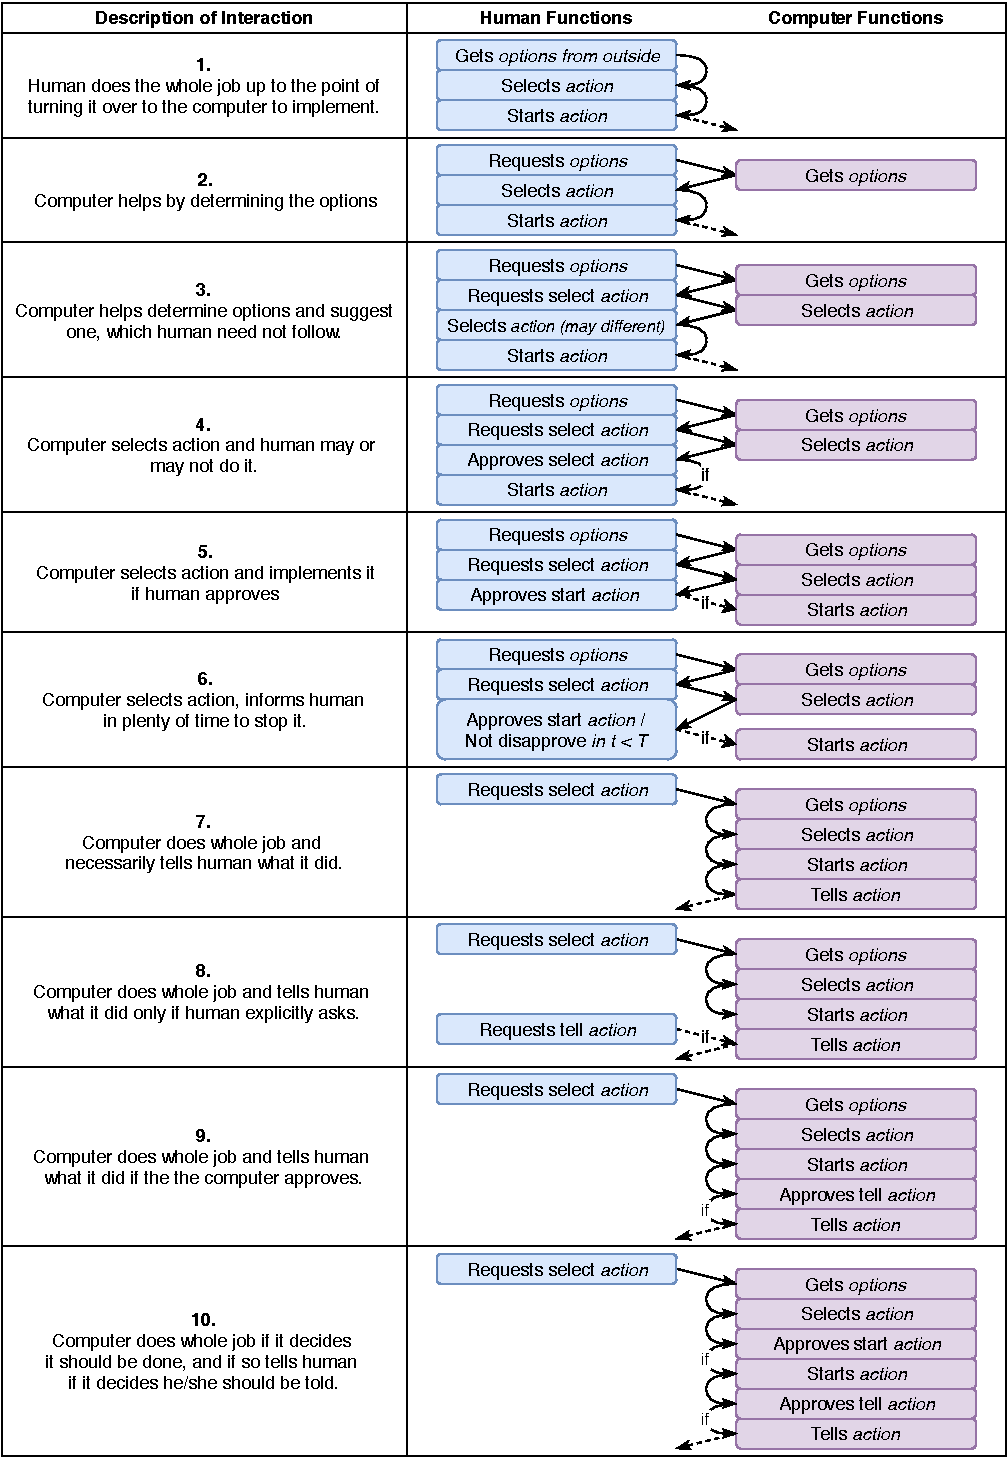
\includegraphics[width=\textwidth]{Figures/draw.io/levels_of_automation_in_man-computer_decision_making_for_a_single_elemental_decisive_step}
    \decoRule
    \caption[Levels of automation in man-computer decision making for a single elemental decisive step]{Levels of automation in man-computer decision making for a single elemental decisive step. \textit{Source: table 8.2 from \cite{Sheridan1978} (edited), created with \href{https://www.draw.io/}{draw.io}}}
    \label{fig:levels_of_automation_in_man-computer_decision_making_for_a_single_elemental_decisive_step}
\end{figure}

%\begin{table}
%    \caption[Levels of Automation in Man-Computer Decision-Making by Sheridan and Verplank]{Levels of Automation in Man-Computer Decision-Making by Sheridan and Verplank. \textit{Source: table 8.2 from \cite{Sheridan1978}, edited.}}
%    \label{tab:Levels_of_Automation_by_Sheridan_and_Verplank}
%    \centering
%    \begin{tabular}{r p{0.8\textwidth} l }
%    \toprule
%    \tabhead{Level} & \tabhead{Definition} \\
%    \midrule
%    1   & The Human remote-controls the UAV and makes all decisions and actions without any assistance from the computer.                      \\
%    2   & The Computer assists the human with decision making by providing a full set of all alternative decisions/actions.                 \\
%    3   & The Computer assists the human with decision making by selecting a subset of alternative decisions/actions.          \\
%    4   & The Computer makes decisions by choosing a single alternative decision/action.                       \\
%    5   & The Computer executes its chosen alternative decision/action, if the human approves.                                     \\
%    6   & The Computer executes its chosen alternative decision/action, if the human does not disapprove in a specified time span.             \\
%    7   & The Computer certainly executes its chosen alternative decision/action and informs the human.                            \\
%    8   & The Computer certainly executes its chosen alternative decision/action and informs the human if he/she requires.                             \\
%    9   & The Computer certainly executes its chosen alternative decision/action and decides whether to inform the human.                             \\
%    10  & The Computer makes all decisions/actions autonomously and ignores the human.                         \\
%    \bottomrule\\
%    \end{tabular}
%\end{table}
% Appendix Template

\chapter{Autonomous Control Levels by Clough} % Main appendix title

\label{AppendixB} % Change X to a consecutive letter; for referencing this appendix elsewhere, use \ref{AppendixX}

\begin{table}
    \tiny
    \caption[Chart of Autonomous Control Levels by Clough]{Chart of Autonomous Control Levels by Clough. \textit{Source: table 4 from \cite{Clough2002}, edited.}}
    \label{tab:chart_of_autonomous_control_levels_by_Clough}
    \centering
    %\begin{adjustbox}{angle=90}
        %\begin{tabular}{r L{0.05\textheight} L{0.18\textheight} L{0.18\textheight} L{0.18\textheight} L{0.18\textheight}}
        \begin{tabular}{r L{0.1\textwidth} L{0.175\textwidth} L{0.175\textwidth} L{0.175\textwidth} L{0.175\textwidth}}
        \toprule
        \tabhead{Lvl} & \tabhead{Label} & \tabhead{Observe} & \tabhead{Orient} & \tabhead{Decide} & \tabhead{Act} \\
        \midrule
        0   & Remotely piloted vehicle                      & Flight control (attitude, rates), sensing, nose camera                                                                                                        & Telemetered data, remote pilot commands                                                                                                                                                                                       & N/A                                                                                                                                           & Control by remote pilot \\
        1   & Execute preplanned mission                    & Preloaded mission data, flight control and navigation sensing                                                                                                 & Pre/post flight BIT, report status                                                                                                                                                                                            & Preprogrammed mission and abort plans                                                                                                         & Wide airspace separation requirements (miles) \\
        2   & Changeable missions                           & Health/status sensors                                                                                                                                         & RT health diagnosis (do I have problems?), offboard replan (as required)                                                                                                                                                      & Execute preprogrammed or uploaded plans in response to mission and health conditions                                                          & Self accomplishment of tactical plan as externally assigned \\
        3   & Robust response to real time faults/events    & Health/status history \& models                                                                                                                               & Tactical plan assigned, RT health diag (what is the extent of the problems?), ability to compensate for most control failures and flight conditions (i.e. adaptive inner-loop control)                                        & Evaluate status vs required mission capabilities, abort/RTB if insufficient                                                                   & Self accomplishment of tactical plan as externally assigned \\
        4   & Fault/event adaptive vehicle                  & Deliberate awareness - allies communicate data                                                                                                                & Tactical plan assigned, assigned rules of engagement, RT health diagnosis, ability to compensate for most control failures and flight conditions - inner loop changes reflected in outer loop performance                     & Onboard trajectory replanning - event driven, self resource management, deconfliction                                                         & Self accomplishment of tactical plan as externally assigned, medium vehicle airspace separation (100's of yds) \\
        5   & Real time multi-vehicle coordination          & Sensed awareness - local sensors to detect others, fused with off-board data                                                                                  & Tactical group plan assigned, RT Health Diagnosis; Ability to compensate for most failures and flight conditions; ability to predict onset of failures (e.g. prognostic health mgmt), group diagnosis and resource management & On-board trajectory replanning - optimizes for current and predictive conditions, collision avoidance                                         & Group accomplishment of tactical plan as externally assigned, air collision avoidance, possible close air space separation (1-100 yds) for AAR, formation in non-threat conditions \\
        6   & Real time multi-vehicle cooperation           & Ranged awareness - on-board sensing for long range, supplemented by off-board data                                                                            & Tactical group goals assigned, enemy location sensed/estimated                                                                                                                                                                & Coordinated trajectory planning and execution to meet goals - group optimization                                                              & Group accomplishment of tactical goal with minimal supervisory assistance, possible close air space separation (1-100 yds) \\
        7   & Battlespace knowledge                         & Short track awareness - history and predictive battlespace data in limited range, timeframe, and numbers, limited inference supplemented by off-board data    & Tactical group goals assigned, enemy trajectory estimated                                                                                                                                                                     & Individual task planning/execution to meet goals                                                                                              & Group accomplishment of tactical goal with minimal supervisory assistance \\
        8   & Battlespace cognizance                        & Proximity inference - intent of self and others (allies and foes), reduced dependance upon off-board data                                                     & Strategic group goals assigned, enemy tactics inferred, ATR                                                                                                                                                                   & Coordinated tactical group planning, individual task planning/execution, choose targets of opportunity                                        & Group accomplishment of strategic goal with minimal supervisory assistance (example: go SCUD hunting) \\
        9   & Battlespace swarm cognizance                  & Battlespace inference - intent of self and others (allies and foes), complex/intense environment - on-board tracking                                          & Strategic group goals assigned, enemy strategy inferred                                                                                                                                                                       & Distributed tactical group planning, individual determination of tactical goal, individual task planning/execution, choose tactical targets   & Group accomplishment of strategic goal with no supervisory assistance \\
        10  & Fully autonomous                              & Cognizant of all within battlespace                                                                                                                           & Coordinates as necessary                                                                                                                                                                                                      & Capable of total indepenance                                                                                                                  & Requires little guidance to do job \\
        \bottomrule\\
        \end{tabular}
    %\end{adjustbox}
\end{table}

% Appendix Template

\chapter{Milestones in UAV Delivery} % Main appendix title

\label{AppendixC} % Change X to a consecutive letter; for referencing this appendix elsewhere, use \ref{AppendixX}


%UPS
%DHL
%Google X
%FedEx
%La Poste
%Alibaba, YTO Express 
%SF Express
%FPS
%CJ Group
%Flirtey
%JD.com
%    This Chinese company is pursuing a massive and rapid expansion of a commercial drone delivery system in the four most-populated provinces in China. 
%    The drones fly from centralized warehouses to locally-designated landing pads. 
%    More than 300,000 local delivery operators then take the packages to the nearby homes. 
%    This company has small commercial drones that can fly up to 62 mph (100 kph) and carry up to 66 lbs. (30 kg). 
%    It also has a very large commercial drone that can carry up to one metric ton (2,200 lbs.). >
%
%DHL
%    In December of 2013, DHL started delivering medicines using drones in Germany. 
%
%Alibaba 
%    In February 2015, Alibaba partnered with the courier company Shanghai YTO Express 
%    to deliver tea by commercial drones to 450 customers in certain Chinese cities. 
%
%Alphabet (Google) 





%\paragraph{Global Timeline of most important events in UAV based delivery}

\begin{table}
    \caption{Timeline - Milestones of developments of UAV based B2C delivery}
    \label{tab:TimelineB2CDelivery}
    \centering
    \begin{tabular}{r r l L{0.15\textwidth} L{0.5\textwidth} l}
    \toprule
    \tabhead{Year} & \tabhead{Month} & \tabhead{Country} & \tabhead{Company} & \tabhead{Details} & \tabhead{Source} \\
    \midrule
    2013    & Dec   & USA       & Amazon                    & Announcement of development \textit{Amazon Prime Air}\cite{AmazonPrimeAir}    &\cite{Manjoo2016} \\
            &       & USA       & UPS                       & research of an own UAV delivery service is announced                          &\cite{Hessinger2013}\\
            &       & Germany   & DHL                       & test delivery flight is conducted                                             &\cite{CBS2013} \\
    2014    & Aug   & Australia & Google X                  & development of \textit{Project Wing} is revealed                              &\cite{Atlantic2014} \\
            & Sep   & Germany   & DHL                       & launch of \textit{Parcelcopter} test program                                  &  \cite{IBTimes2014-09}  \\
            & Oct   & USA       & FedEx                     & research of UAV integration into existing delivery system is announced        &\cite{IBTimes2014} \\       
            & Dec   & France    & La Poste                  & launch of test program                                                        & \cite{Telegraph2014} \\
    2015    & Feb   & China     & Alibaba, YTO Express      & launch of tea delivery program                                                &\cite{BusinessInsider2015}\\
            & Mar   & China     & SF Express                & launch of test UAV delivery service                                           &\cite{Xaircraft} \\
            &       & UK        & FPS                       & First commercial UAV delivery in the UK                                       & \cite{FPS2015} \\
            & May   & Korea     & CJ Group                  & development on UAV delivery system is revealed                                & \cite{PostnParcel2015} \\
            & Jul   & USA       & Flirtey                   & First commercial UAV delivery in the US                                       &\cite{Flirtey2015} \\
    2016    & Jul   & USA       & 7-Eleven, Flirtey         & first "store-to-door" UAV deliveries to private customers in the US with an autonomously flying drone relying on precision GPS & \cite{PostnParcel}\\
            %& Oct   &
            & Dec   & UK        & Amazon                    & first UAV delivery in the United Kingdom                                      &  \cite{Amazon2016} \\
    2017    & Aug   & Iceland   & Aha, Flytrex, DJI         & launched a project to fly drones preprogrammed missions to deliver consumer goods to customers' houses in Rejkjavik & \cite{Ross2018} \\
            
    \bottomrule\\
    \end{tabular}
\end{table}




%The concept of commercial UAV delivery started in 2013 when Amazon announced the initiative "Amazon Prime Air"\cite{AmazonPrimeAir}
%to develope UAV systems for parcel delivery.\cite{Manjoo2016}
%Within less than a week, UPS reacted on the plans of Amazon to enter the core business of UPS by announcing own plans for UAV delivery.\cite{Hessinger2013}
%Nevertheless, in the shadow of these gigantic companies, in July 2015 Flirtey, an Australian start-up, 
%conducted the first federally-approved commercial UAV delivery in the United States.\cite{Flirtey2015}
%Thereupon, in July 2016 Flirtey in corporation with 7-Eleven, a large internationally operating chain of convenience stores, 
%performed the first "store-to-door" UAV deliveries to private customers in the US with an autonomously flying drone relying on precision GPS.\cite{PostnParcel}
%October 2016 Zipline
%In December 2016, Amazon caught up with its first UAV delivery in the United Kingdom \cite{Amazon2016},
%where legal regulations with respect to autonomously flying UAVs are less restrictive than in the United States. \cite{DailyCaller2017}
%In August 2017,  Aha in corporation with Flytrex, start-ups from Iceland and Israel, respectively, 
%launched a project to fly drones manufactured by DJI on preprogrammed missions to deliver consumer goods to customers' houses in Rejkjavik, the capital of Iceland. 
%Iceland previously relaxed necessary regulations for this project.\cite{Ross2018}








%CHINA
%With its huge population (1.4 billion people in 2018)
%eCommerce Report
%and broad social acceptance towards digital innovations
%-in comparison 39\% of US American citizens
%are sceptical towards drone delivery
%https://www.statista.com/chart/5843/level-of-trust-in-drone-delivery-services/-,
%China surpassed the United States of America in 2013 and
%became the biggest eCommerce market worldwide with
%a total revenue of approximately 633.9 billion USD in 2018
%leaving the US on second place with 501.0 billion USD and 
%the European Union on third place with 358.1 billion USD.
%eCommerce Report
%https://www.techinasia.com/2013-china-surpasses-america-to-become-worlds-top-ecommerce-market
%https://www.statista.com/study/42335/ecommerce-report/
%The growth of eCommerce has strong impact on the logistics market demanding innovative and efficient approaches
%for fast and reliable door step parcel delivery shipment even in remote areas with little infrastructure.
%logistic companies.
%The China-based companies DJI, ... are among the biggest drone developers and producers
%and came up with highly engineered, innovative drone systems.
%For individuals as well as in corporation with the
%dominating shipment companies JD, SF Express, in China.
%Several China-based companies 
%are testing drone delivery supported by
%innovative drone comanies such as DJI.
%https://www.scmp.com/tech/innovation/article/2129585/jdcoms-autonomous-delivery-vehicles-will-take-streets-tianjin-june
%After the approval by the China Civil Aviation Administration
%<build tens of thousands UAV landing platforms or drone pods across China>
%JD.com extended its drone projects
%with own UAV, unmanned ground vehicles, and unmanned warehouses
%within its JDX Department for intelligent logistics.
%https://technode.com/2018/02/05/e-commerce-giant-jd-will-build-tens-of-thousands-delivery-drone-landing-pods/
%https://jdcorporateblog.com/jd-com-announces-series-of-new-agreements-for-drone-development/
%https://jdcorporateblog.com/jd-com-to-build-largest-drone-logistics-network-and-rd-campus-in-china/
%While the logistics subsidiary of JD.com
%which is the second biggest business to customer (B2C) eCommerce company
%in China after Tmall of the Alibaba Group
%%https://www.statista.com/statistics/959881/china-gmv-share-of-online-retail-b2c-market-by-platform/
%was opening its first UAV distribution center in Haikou, the capital of Hainan in 2018,
%the first company that received a license for drone delivery services
%by responsible Chinese administration was Jiangxi Fengyu Shuntu Technology Company.
%%https://technode.com/2018/03/28/first-licence-for-drone-deliveries-in-china-goes-to-sf-express/
%%http://www.xinhuanet.com/finance/2018-03/28/c_1122600619.htm
%The company is an affiliated company of SF Express 
%which is one of the biggest delivery service companies in China 
%%https://www.statista.com/statistics/244034/leading-logistics-companies-in-china-by-revenue/
%An airborne supply chain consisting of nationwidely operating planes,
%locally distributing larger drones and customer delivering smaller drones
%should foremost increase the coverage of delivery and
%the delivery time in rural areas.
%%https://technode.com/2018/03/28/first-licence-for-drone-deliveries-in-china-goes-to-sf-express/
%
%
%
%<
%Its first drone took off on 26 March on its way to the company’s first Hainan delivery (in Chinese). 
%Hainan is an island off the southern coast of the mainland and is highly mountainous and so a suitable testing ground for the format. 
%JD has ambitions to be able to deliver anywhere in the country within 24 hours.>
%%http://tech.sina.com.cn/i/2018-03-26/doc-ifysqfnh0749009.shtml
%%https://jdcorporateblog.com/jd-com-launches-new-institute-for-smart-logistics-in-urban-areas-2/
%
%
%
%International
%Corporation with Rakuten in Japan
%%https://jdcorporateblog.com/jd-com-and-rakuten-to-collaborate-on-unmanned-delivery-solutions-in-japan/
%Indonesia
%%https://jdcorporateblog.com/gallery/jd-com-launches-first-government-approved-drone-flight-in-indonesia-2/
%
%
%
%
%


%e-commerce giant JD.com and delivery giant SF Holding %https://www.bloomberg.com/news/features/2018-07-03/china-s-on-the-fast-track-to-making-uav-drone-deliveries
%
%
%
%
%
%
%
%
%
%already capable of being deployed for many types of delivery services 
%such as pizzas in urban environments and 
%desperately-needed medicine flown by drones to remote inaccessible villages.
%%https://spectrum.ieee.org/robotics/drones/in-the-air-with-ziplines-medical-delivery-drones
%
%
%
%5G technology providing high bandwidth and low latency takes a crucial position in the safe navigation of autonomous UAVs.\cite{Bianji2019}
%The fast transfer of data and high definition videos will enable UAV systems in many commercial applications.
%
%
%
%
%%Regulations
%
%FAA rules currently prohibit drone flights 
%that are entirely autonomous or 
%beyond the line of sight of human operators.
%
%regulatory: autonomous systems in which multiple aircraft are overseen by one pilot, fly beyond the vision of that pilot. 
%    Current regulations do not permit multiple drones per operator without a waiver
%
%
%%Technical
%
%
%currently only transport parcels of up to ~ 5 kg
%landing areas of at least 2 m2.
%%https://www.mckinsey.com/~/media/mckinsey/industries/travel%20transport%20and%20logistics/our%20insights/how%20customer%20demands%20are%20reshaping%20last%20mile%20delivery/parcel_delivery_the_future_of_last_mile.ashx
%battery
%https://ieeexplore.ieee.org/abstract/document/7934790
%
%
%saftey: fly beyond a pilot’s visual line of sight, to operate at night and to fly over people.\cite{Rosen2019}
%
%
%%-----------------
%%LINKS
%
%
%DHL
%%https://www.dpdhl.com/en/media-relations/specials/dhl-parcelcopter.html
%%https://discover.dhl.com/business/business-ethics/parcelcopter-drone-technology
%%https://polygon-design.com/en/references/projects/_projects/dhlparcelcopter-skyport.html
%%https://www.dhl.de/en/privatkunden/pakete-empfangen/an-einem-abholort-empfangen/packstation-empfang.html
%
%
%Domino first Pizza
%%https://www.youtube.com/watch?v=JoP1lvgGLys
%%https://money.cnn.com/2016/08/26/technology/dominos-drone-new-zealand/?iid=EL
%
%UPS
%%https://www.businessinsider.de/ups-tests-drone-delivery-system-2017-2?r=US&IR=T
%%https://www.theverge.com/2019/7/23/20707470/ups-drone-delivery-faa-certification-approval
%%https://www.fleetowner.com/technology/ups-sets-new-milestone-drone-delivery-services
%
%
%Google, X Development, Project Wing
%%https://x.company/projects/wing/
%%https://wing.com/finland/helsinki/
%%https://www.bloomberg.com/news/articles/2019-04-23/alphabet-s-drone-delivery-business-cleared-for-takeoff-by-faa
%%https://money.cnn.com/2016/09/08/technology/google-drone-chipotle-burrito/?iid=EL
%
%Amazon Air Prime
%%https://www.washingtonpost.com/news/the-switch/wp/2013/12/01/amazon-wants-to-deliver-packages-in-30-minutes-with-drones/
%%https://www.bbc.com/news/technology-38320067
%%https://www.forbes.com/sites/colinsnow/2019/06/17/amazons-drone-delivery-whats-old-whats-new-and-when/#22896c935f91
%
%
%Flytrex, AHA in Iceland
%%https://www.washingtonpost.com/news/innovations/wp/2017/08/25/you-can-now-hav
%%https://ecommerceguide.com/news/aha-flytrex-team-offer-drone-delivery-iceland/
%
%
%Boeing
%%https://www.flightglobal.com/news/articles/unmanned-cargo-lifter-deepens-boeings-push-on-auton-444788/
%
%
%JD.com
%%http://unmannedcargo.org/chinese-delivery-drones/
%%https://www.bloomberg.com/news/features/2018-07-03/china-s-on-the-fast-track-to-making-uav-drone-deliveries
%
%Zipline
%%https://www.flyzipline.com/
%%https://www.nytimes.com/2016/04/05/technology/drones-marshaled-to-drop-lifesaving-supplies-over-rwandan-terrain.html?module=inline
%
%Swoop Aero
%%https://swoop.aero/
%%https://www.nytimes.com/2018/12/17/health/vanuatu-vaccines-drones.html?module=inline
%
%UAS Integration Pilot Program
%%https://www.faa.gov/uas/programs_partnerships/integration_pilot_program/
%
%European Union’s test of drone deliveries
%%https://www.nytimes.com/2018/12/31/business/europe-commercial-drone-delivery.html?module=inline
%
%Matternet
%%https://mttr.net/product
%
%University of Alaska Fairbanks
%%https://www.reuters.com/article/us-usa-faa-drones/first-u-s-faa-approved-beyond-line-of-sight-drone-flight-completed-idUSKCN1US2LR
%
%
%General
%%https://uavcoach.com/drone-deliveries-2018/
%%https://jrupprechtlaw.com/amazon-drone-delivery-3-major-legal-problems-amazon-prime-air/
%%https://mydroneauthority.com/industry/drone-delivery/

%----------------------------------------------------------------------------------------
%	BIBLIOGRAPHY
%----------------------------------------------------------------------------------------

\printbibliography[heading=bibintoc]

%----------------------------------------------------------------------------------------

\end{document}  
